\chapter{变分视角：从VAE到DDPM}\label{ch:variational}


在本章中，我们通过变分透镜来观察扩散模型。我们从变分自编码器（VAE）开始，它表示具有潜变量的数据，并通过最大化对数似然的易处理下界来进行训练。在这种设置中，学习的编码器将观察结果映射到潜变量，学习的解码器将潜变量映射回观察结果，从而关闭建模循环。 

在此模式的基础上，分层变体（分层 VAE）堆叠多个潜在层以捕获多个尺度的结构。通过这种设置，去噪扩散概率模型（DDPM）在概念上遵循类似的模板：编码器被固定为逐渐将数据映射到噪声的前向噪声过程，而不是联合训练编码器和解码器，并且训练学习在连续的去噪步骤中反转该路径的解码器。从这个角度来看，VAE、分层 VAE 和扩散模型都优化了由变分界定义的似然代理，为这里介绍的方法提供了共同的基础。

\chapterlearning{
  \item 了解为什么当精确的最大似然训练很困难时，VAE 会优化 ELBO；
  \item 了解 DDPM 如何将 VAE 的潜变量视图扩展到许多噪声层，并具有固定的噪声过程和学习的逆过程；
  \item 了解将困难的反向降噪问题转化为易于处理的训练目标的条件技巧；
  \item 比较均值、干净数据和噪声预测，并了解它们如何表示相同的底层去噪信息；
  \item 通过 ELBO 将实际的 DDPM 去噪损失连接回其变分基础。
}{
已经熟悉 VAE 和 ELBO 训练的读者可以浏览 \Cref{sec:vae} 并从 \Cref{sec:ddpm} 开始。
}



\newpage
\section{变分自编码器}\label{sec:vae}
神经网络如何学习生成真实数据？  
一个自然的起点是 \emph{autoencoder}，它由两个网络组成：  
确定性 \emph{encoder} 将输入压缩为低维潜在代码，确定性 \emph{decoder} 从此代码重建输入。  
训练最小化原始输入与其重建之间的重建误差。  
虽然这种设置可以实现准确的重建，但潜在空间是非结构化的：随机采样潜在代码通常会产生无意义的输出，限制了模型的生成用途。





\emph{变分自编码器 (VAE)} \citep{kingma2013auto} 通过在潜在空间上施加概率结构来解决这个问题。这将模型从简单的重建工具转变为真正的生成模型，能够生成新颖且真实的数据。



\subsection{概率编码器和解码器}

\begin{figure}[tbh!]
\centering
\resizebox{0.85\linewidth}{!}{
\begin{tikzpicture}[>=Latex, thick, font=\sffamily, node distance=0.8cm]

\tikzset{
  state/.style={
    rectangle, rounded corners=3pt,
    draw=black, fill=gray!10,
    minimum height=45pt, minimum width=25pt, align=center,
    % Add outer sep to ensure arrows connect cleanly to the rounded edges
    outer sep=0pt 
  },
  latent/.style={
    rectangle, rounded corners=3pt,
    draw=black, fill=gray!10,
    minimum height=28pt, minimum width=28pt, align=center,
    outer sep=0pt
  },
  encoderblock/.style={
    trapezium, trapezium stretches=true,
    % Adjust angles to create the frustum shape.
    % The 'top' and 'bottom' here refer to the sides that become the vertical parallels after rotation.
    trapezium left angle=80,  % Closer to 90 for less slope
    trapezium right angle=80, % Closer to 90 for less slope
    shape border rotate=270,   % Rotate 90 degrees clockwise for vertical parallels
    draw=black, fill=gray!20,
    minimum height=8pt, minimum width=15pt, inner sep=4pt, align=center
  },
  decoderblock/.style={
    trapezium, trapezium stretches=true,
    trapezium left angle=80,
    trapezium right angle=80,
    shape border rotate=90,  % Rotate 270 degrees clockwise (or -90)
    draw=black, fill=gray!20,
    minimum height=8pt, minimum width=15pt, inner sep=4pt, align=center
  }
}

% nodes
\node[state] (x) {$\mathbf{x}$};
\node[encoderblock, right=of x] (enc) {\footnotesize\textbf{Encoder}\\[-2pt]
 \footnotesize $q_{\bm{\theta}}(\mathbf{z}|\mathbf{x})$}; % Using bm for bold math
\node[latent, right=of enc] (z) {$\mathbf{z}$};
\node[decoderblock, right=of z] (dec) {\footnotesize\textbf{Decoder}\\[-2pt]
  \footnotesize$p_{\bm{\phi}}(\mathbf{x}|\mathbf{z})$}; % Using bm for bold math
\node[state, right=of dec] (xprime) {$\mathbf{x}'$};

% short arrows (edge-to-edge)
\draw[->] (x) -- (enc); % Changed to direct node-to-node, TikZ usually finds the nearest edge
\draw[->] (enc) -- (z);
\draw[->] (z) -- (dec);
\draw[->] (dec) -- (xprime);

\end{tikzpicture}}
\caption{\textbfs{VAE 插图。} 由随机编码器组成 $q_{\bm{\theta}}(\rvz|\rvx)$ 映射数据 $\rvx$ 到潜变量 $\rvz$和解码器 $p_{\bm{\phi}}(\rvx|\rvz)$ 从潜在数据中重建数据。 \figcredit{由作者创建。}}
\label{fig:vae-graph}
\end{figure}

\paragraph{解码器（生成器）的构造。}










在 VAE 中，我们区分两种类型的变量： 
\emph{观察到的变量} $\rvx$，对应于我们看到的数据（例如图像），以及 \emph{潜变量} $\rvz$，捕获变化的隐藏因素（例如，对象形状、颜色或样式）。该模型假设每个观察 $\rvx$ 是从简单样本中采样的潜变量生成的 \emph{先验分布}，通常是标准高斯， 
$\rvz \sim p_{\text{prior}} := \mathcal{N}(\mathbf{0}, \mathbf{I})$。前往映射 $\rvz$ 回到数据空间，我们定义一个 \emph{解码器（发生器）} 分布 
$p_{\bm{\phi}}(\rvx|\rvz)$。在实践中，这个解码器保持简单，通常是因式分解的高斯（参见 \Cref{subsec:optimization-vae}) 或类似的分布，以便学习专注于提取有用的潜在特征而不是记忆数据。直观上，直接一一生成像素是极其困难的；相反，潜变量提供了一种紧凑的表示，从中解码精确的像素排列变得更加容易。通过第一次采样抽取新样本 $\rvz \sim p_{\text{prior}}$ 然后通过解码 $\rvx \sim p_{\bm{\phi}}(\rvx|\rvz)$。因此，VAE 通过边缘似然定义了一个潜变量生成模型：
\[
p_{\bm{\phi}}(\rvx) = \int p_{\bm{\phi}}(\rvx|\rvz) p(\rvz) \diff \rvz.
\]
理想情况下，解码器参数 $\bm{\phi}$ 通过最大化边缘似然来学习，如最大似然估计（参见 \Cref{eq:MLE}）。然而，由于积分超过 $\rvz$ 对于富有表现力的非线性解码器来说是棘手的，直接 MLE 在计算上不可行，这激发了 VAE 中使用变分方法。





\paragraph{编码器（推理网络）的构建。}














要将我们棘手的生成器连接到真实数据，请考虑相反的问题：给定一个观察结果 $\rvx$，什么隐藏代码 $\rvz$ 可以生产吗？根据贝叶斯法则，后验分布为
\[
p_{\bm{\phi}}(\rvz|\rvx) \;=\; \frac{p_{\bm{\phi}}(\rvx|\rvz) p(\rvz)}{p_{\bm{\phi}}(\rvx)}.
\]
困难在于分母涉及边缘似然 $p_{\bm{\phi}}(\rvx)$，这需要对所有潜变量进行积分，并且对于非线性解码器来说是棘手的。因此，精确推断 $\rvz$ 来自 $\rvx$ 计算量巨大。

VAE 中的“变分”步骤通过用易于处理的近似替换难以处理的后验来解决这个问题。我们介绍一个 \emph{编码器} （或推理网络） $q_{\bm{\theta}}(\rvz|\rvx)$，由神经网络参数化，其作用是充当可学习的代理：
\[
q_{\bm{\theta}}(\rvz|\rvx) \;\approx\; p_{\bm{\phi}}(\rvz|\rvx).
\]
实际上，编码器映射每个观察到的数据点 $\rvx$ 潜在代码的分布，提供可行且可训练的途径 $\rvx$ 返回 $\rvz$ 支持学习。




\subsection{通过证据下界 (ELBO) 进行训练}

我们现在定义一个可计算的训练目标。虽然我们无法直接优化 $\log p_{\bm{\phi}}(\mathbf{x})$，我们可以最大化它的下界—— \emph{证据下限 (ELBO)}:

\thmp{证据下限 (ELBO)}{elbo}{
对于任何数据点 $\mathbf{x}$，对数似然满足：
\[
\log p_{\bm{\phi}}(\mathbf{x}) \geq \mathcal{L}_{\text{ELBO}}(\bm{\theta}, \bm{\phi}; \mathbf{x}),
\]
其中 ELBO 由以下公式给出： 
\begin{align}\label{eq:vae-elbo}
    \mathcal{L}_{\text{ELBO}} = \underbrace{\mathbb{E}_{\mathbf{z} \sim q_{\bm{\theta}}(\mathbf{z}|\mathbf{x})} \left[ \log p_{\bm{\phi}}(\mathbf{x}|\mathbf{z}) \right]}_{\text{Reconstruction Term}} - \underbrace{\mathcal{D}_{\mathrm{KL}}\left( q_{\bm{\theta}}(\mathbf{z}|\mathbf{x}) \| p(\mathbf{z}) \right)}_{\text{Latent Regularization}}.
\end{align}
}{
ELBO 由 Jensen 不等式产生：
\begin{align*}
\log p_{\bm{\phi}}(\mathbf{x}) &= \log \int p_{\bm{\phi}}(\mathbf{x}, \mathbf{z})   \mathrm{d}\mathbf{z} = \log \int q_{\bm{\theta}}(\mathbf{z}|\mathbf{x}) \frac{p_{\bm{\phi}}(\mathbf{x}, \mathbf{z})}{q_{\bm{\theta}}(\mathbf{z}|\mathbf{x})}   \mathrm{d}\mathbf{z} \\
&= \log \mathbb{E}_{\mathbf{z} \sim q_{\bm{\theta}}(\mathbf{z}|\mathbf{x})} \left[ \frac{p_{\bm{\phi}}(\mathbf{x}, \mathbf{z})}{q_{\bm{\theta}}(\mathbf{z}|\mathbf{x})} \right] \geq \mathbb{E}_{\mathbf{z} \sim q_{\bm{\theta}}(\mathbf{z}|\mathbf{x})} \left[ \log \frac{p_{\bm{\phi}}(\mathbf{x}, \mathbf{z})}{q_{\bm{\theta}}(\mathbf{z}|\mathbf{x})} \right].
\end{align*}
}
ELBO 目标自然分解为两部分：
\begin{itemize}
    
    
    \item \textbfs{重建：} 鼓励准确恢复 $\mathbf{x}$ 来自其隐藏代码 $\mathbf{z}$。通过高斯编码器和解码器假设，该项精确地减少到熟悉的自动编码器的重建损失（参见\ \Cref{subsec:optimization-vae}）。然而，就像在自动编码器中一样，单独优化这项有可能会记住训练数据，从而引发额外的正则化。
    \item \textbfs{潜在 KL：} 鼓励编码器分发 $q_{\bm{\theta}}(\mathbf{z}|\mathbf{x})$ 接近简单的高斯先验 $p_{\mathrm{prior}}(\mathbf{z})$。这种正则化将潜在空间塑造成平滑且连续的结构，通过确保从先验中提取的样本可以被可靠地解码，从而实现有意义的生成。
\end{itemize}
这种权衡确保了忠实的重建和相干的采样。

\paragraph{信息理论观点：ELBO 作为散度界。}







































ELBO 目标具有自然的信息论解释。回想一下，最大似然训练相当于最小化 KL 散度
\[
\mathcal{D}_{\mathrm{KL}}(p_{\text{data}}(\rvx) \| p_{\bm{\phi}}(\rvx)),
\]
衡量模型分布与数据分布的近似程度。由于该术语通常很难处理，因此变分框架引入了联合比较。具体来说，考虑两个联合分布：
\begin{itemize}
    \item 这 \textbfs{生成关节}, $p_{\bm{\phi}}(\rvx, \rvz) = p(\rvz) p_{\bm{\phi}}(\rvx|\rvz)$，描述了模型如何生成数据；
    \item 这 \textbfs{推理关节}, $q_{\bm{\theta}}(\rvx, \rvz) = p_{\text{data}}(\rvx) q_{\bm{\theta}}(\rvz|\rvx)$，它将真实数据与其推断的潜在数据相结合。
\end{itemize}
比较这些分布会产生不等式
\begin{align}\label{eq:joint-bound}
    \mathcal{D}_{\mathrm{KL}}(p_{\text{data}}(\rvx) \| p_{\bm{\phi}}(\rvx)) 
    \leq \mathcal{D}_{\mathrm{KL}}(q_{\bm{\theta}}(\rvx,\rvz) \| p_{\bm{\phi}}(\rvx,\rvz)),
\end{align}
有时称为 KL 散度的链式法则。直观上，仅比较边缘值（$\rvx$) 可以隐藏在考虑完整潜在数据联合时显示的不匹配。形式上，我们可以将联合 KL 扩展为
\begin{align*}
    &\underbrace{\mathcal{D}_{\mathrm{KL}}(q_{\bm{\theta}}(\mathbf{x}, \mathbf{z}) \| p_{\bm{\phi}}(\mathbf{x}, \mathbf{z}))}_{\text{Total Error Bound}} 
    \\=& \mathbb{E}_{q_{\bm{\theta}}(\mathbf{x}, \mathbf{z})} \left[ \log \frac{p_{\text{data}}(\mathbf{x}) q_{\bm{\theta}}(\mathbf{z}|\mathbf{x})}{p_{\bm{\phi}}(\mathbf{x}) p_{\bm{\phi}}(\mathbf{z}|\mathbf{x})} \right] \\=&\mathbb{E}_{p_{\text{data}}(\mathbf{x})} \left[ \log \frac{p_{\text{data}}(\mathbf{x})}{p_{\bm{\phi}}(\mathbf{x})} + \mathcal{D}_{\mathrm{KL}}\left( q_{\bm{\theta}}(\mathbf{z}|\mathbf{x}) \| p_{\bm{\phi}}(\mathbf{z}|\mathbf{x}) \right) \right] \\
    \\=&  \underbrace{\mathcal{D}_{\mathrm{KL}}(p_{\text{data}} \| p_{\bm{\phi}})}_{\text{True Modeling Error}} + \underbrace{\mathbb{E}_{p_{\text{data}}(\mathbf{x})} \big[ \mathcal{D}_{\mathrm{KL}}( q_{\bm{\theta}}(\mathbf{z}|\mathbf{x}) \| p_{\bm{\phi}}(\mathbf{z}|\mathbf{x}) ) \big]}_{\text{Inference Error}},
\end{align*}
其中第一项是真实的建模误差，第二项是推理误差，即近似后验和真实后验之间的差距。后者始终为非负数，这解释了 \Cref{eq:joint-bound}。

最后，请注意
\[
\log p_{\bm{\phi}}(\rvx) - \mathcal{L}_{\text{ELBO}}(\bm{\theta},\bm{\phi};\rvx) 
= \mathcal{D}_{\mathrm{KL}} \left(q_{\bm{\theta}}(\rvz|\rvx)\|p_{\bm{\phi}}(\rvz|\rvx)\right).
\]
因此，推理误差正是对数似然与 ELBO 之间的差距。 
因此，最大化 ELBO 相当于直接减少推理错误，确保训练最小化总体界限的有意义部分。












































\subsection{高斯VAE}\label{subsec:optimization-vae}
VAE 的标准公式对编码器和解码器都采用高斯分布。
\paragraph{编码器零件}
编码器 $ q_{\bm{\theta}}(\mathbf{z} | \mathbf{x}) $ 通常被建模为高斯分布：
\[
q_{\bm{\theta}}(\mathbf{z} | \mathbf{x}) := \mathcal{N}\left(\mathbf{z}; \bm{\mu}_{\bm{\theta}}(\mathbf{x}), \operatorname{diag}(\bm{\sigma}_{\bm{\theta}}^2(\mathbf{x}))\right),
\]
其中 $\bm{\mu}_{\bm{\theta}} : \mathbb{R}^D \to \mathbb{R}^d$ 和 $\bm{\sigma}_{\bm{\theta}} : \mathbb{R}^D \to \mathbb{R}_+^d$ 是编码器网络的确定性输出。
\paragraph{Decoder Part.} 解码器通常建模为具有固定方差的高斯分布：
\[
p_{\bm{\phi}}(\mathbf{x}|\mathbf{z}) := \mathcal{N}\bigl(\mathbf{x}; \bm{\mu}_{\bm{\phi}}(\mathbf{z}), \sigma^2 \rmI\bigr),
\]
其中$\bm{\mu}_{\bm{\phi}} : \mathbb{R}^d \to \mathbb{R}^D$是一个神经网络，$\sigma > 0$是一个控制方差的小常数。
 
在此假设下，ELBO 中的重建项简化为
\[
\mathbb{E}_{q_{\bm{\theta}}(\mathbf{z} | \mathbf{x})} \left[\log p_{\bm{\phi}}(\mathbf{x} | \mathbf{z})\right]
= - \frac{1}{2\sigma^2} \mathbb{E}_{q_{\bm{\theta}}(\mathbf{z} | \mathbf{x})} \left[\|\mathbf{x} - \bm{\mu}_{\bm{\phi}}(\mathbf{z})\|^2\right] + C,
\]
其中 $C$ 是独立于 $\bm{\theta}$ 和 $\bm{\phi}$ 的常数。因此，ELBO 目标简化为：
\[
\min_{\bm{\theta}, \bm{\phi}}  \mathbb{E}_{q_{\bm{\theta}}(\mathbf{z} | \mathbf{x})} \left[ \frac{1}{2\sigma^2} \|\mathbf{x} - \bm{\mu}_{\bm{\phi}}(\mathbf{z})\|^2 \right]
+ \mathcal{D}_{\mathrm{KL}}\big(q_{\bm{\theta}}(\mathbf{z} | \mathbf{x}) \| p_{\mathrm{prior}}(\mathbf{z})\big),
\]
其中，由于高斯假设，KL 项承认封闭式解。因此，训练 VAE 可以减少正则化重建损失的最小化。

\subsection{标准VAE的缺点}\label{sec:drawback_standard_VAE}
尽管 VAE 框架在理论上很有吸引力，但它有一个严重的缺点：它经常产生模糊的输出\footnote{我们在这里研究的限制特定于引入的常见 VAE 设置
上图：通过平方重建训练的简单高斯解码器
错误。在此设置中，群体最优解码器返回一个条件
意思是。如果几个视觉上不同的输入对应于重叠的潜在
区域，这种平均可能会显得模糊。这不应被解读为
关于每个 VAE 架构或观察模型的通用声明。}。

\paragraph{ VAE 中的模糊生成。}
为了理解这种现象，考虑一个固定的高斯编码器 $ q_{\text{enc}}(\mathbf{z}|\mathbf{x}) $ 和一个以下形式的解码器
\[
p_{\text{dec}}(\mathbf{x}|\mathbf{z}) = \mathcal{N}(\mathbf{x}; \bm{\mu}(\rvz), \sigma^2 \rmI),
\]
其中 $ \bm{\mu}(\rvz) $ 表示解码器网络。使用任意编码器，优化 ELBO 可减少（最多可达加性常数）以最小化预期重建误差：
\[
\argmin_{\bm{\mu}} \mathbb{E}_{p_{\text{data}}(\mathbf{x})q_{\text{enc}}(\mathbf{z}|\mathbf{x})} \left[ \| \mathbf{x} - \bm{\mu}(\rvz) \|^2 \right].
\]
这是 $ \bm{\mu}(\rvz) $ 中的标准最小二乘问题，其解由条件均值以封闭形式给出：
\[
\bm{\mu}^*(\mathbf{z}) = \mathbb{E}_{q_{\text{enc}}(\mathbf{x}|\mathbf{z})}[\mathbf{x}],
\]
其中 $ q_{\text{enc}}(\mathbf{x}|\mathbf{z}) $ 是给定潜在输入的编码器诱导后验，通过贝叶斯规则定义：
\[
q_{\text{enc}}(\mathbf{x}|\mathbf{z})
=
\frac{q_{\text{enc}}(\mathbf{z}|\mathbf{x})\, p_{\text{data}}(\mathbf{x})}{q_{\text{enc}}(\mathbf{z})},
\qquad
q_{\text{enc}}(\mathbf{z})
:=
\int q_{\text{enc}}(\mathbf{z}|\mathbf{x})\, p_{\text{data}}(\mathbf{x})\, \diff \mathbf{x}.
\]通过贝叶斯规则的最优生成器的等效形式是：
\[
\bm{\mu}^*(\mathbf{z})
=
\frac{\mathbb{E}_{p_{\text{data}}(\mathbf{x})}\!\left[q_{\text{enc}}(\mathbf{z}|\mathbf{x}) \cdot \mathbf{x}\right]}
{q_{\text{enc}}(\mathbf{z})}
=
\frac{\mathbb{E}_{p_{\text{data}}(\mathbf{x})}\!\left[q_{\text{enc}}(\mathbf{z}|\mathbf{x}) \cdot \mathbf{x}\right]}
{\mathbb{E}_{p_{\text{data}}(\mathbf{x})}\!\left[q_{\text{enc}}(\mathbf{z}|\mathbf{x})\right]}.
\]
现在假设两个不同的输入 $ \mathbf{x} \neq \mathbf{x}' $ 映射到潜在空间中的重叠区域，即 $ q_{\text{enc}}(\cdot|\mathbf{x}) $ 和 $ q_{\text{enc}}(\cdot|\mathbf{x}') $ 的支撑相交。然后 $\bm{\mu}^*(\mathbf{z})$ 对多个可能不相关的输入进行平均，这会导致模糊、不明确的输出。这种对冲突模式的平均效应是 VAE 生成的样本特征模糊的根本原因。




\newpage
\subsection{（选读）从标准VAE到分层VAE}
为了对复杂数据进行建模，分层变分自编码器 (HVAE)
\citep{vahdat2020nvae} 通过引入潜变量层次结构来增强 VAE。这种深层的分层结构使模型能够捕获多个抽象级别的数据特征，从而显着增强表达能力并反映现实世界数据的组成性质。
\vspace{0.3cm}
\begin{figure}[tbh!]
    \centering
\begin{tikzpicture}[
    ->, % Sets default arrow type
    >=Stealth, % Sets default arrowhead style
    node_dist/.style={right=1.7cm of #1}, % Style for node distance
    font=\small,
    thick
  ]

  % Define a style for the circular nodes
  \tikzset{state/.style={
      rectangle,
      rounded corners=3pt,
      draw=black,
      fill=gray!10,
      minimum height=35pt,
      minimum width=25pt
    }
  }

  % Place the nodes
  \node[state] (x) {$\rvx$};
  \node[state] (z1) [node_dist=x] {$\rvz_1$};
  \node[state] (z2) [node_dist=z1] {$\rvz_2$};
  \node (dots) [right=0.7cm of z2] {$\boldsymbol{\cdots}$};
  \node[state] (zT) [node_dist=dots] {$\rvz_L$};

  % Draw the arrows (edges) with labels
  
  % Inference path (top, q, forward) - Shifted up
  \path ([yshift=4.5pt]x.east)  edge node[above] {$q_{\bm{\theta}}(\rvz_1|\rvx)$} ([yshift=4.5pt]z1.west);
  \path ([yshift=4.5pt]z1.east) edge node[above] {$q_{\bm{\theta}}(\rvz_2|\rvz_1)$} ([yshift=4.5pt]z2.west);
  \path ([yshift=4.5pt]z2.east) edge ([yshift=4.5pt]dots.west);
  % --- CHANGED: Added pos=0.4 to shift label left ---
  \path ([yshift=4.5pt]dots.east) edge node[above, pos=0.4] {$q_{\bm{\theta}}(\rvz_L|\rvz_{L-1})$} ([yshift=4.5pt]zT.west);
  
  % Generative path (bottom, p, backward) - Shifted down
  \path ([yshift=-4.5pt]z1.west) edge node[below] {$p_{\bm{\phi}}(\rvx|\rvz_1)$} ([yshift=-4.5pt]x.east);
  \path ([yshift=-4.5pt]z2.west) edge node[below] {$p_{\bm{\phi}}(\rvz_1|\rvz_2)$} ([yshift=-4.5pt]z1.east);
  \path ([yshift=-4.5pt]dots.west) edge ([yshift=-4.5pt]z2.east);
  % --- CHANGED: Added pos=0.6 to shift label left ---
  \path ([yshift=-4.5pt]zT.west) edge node[below, pos=0.6] {$p_{\bm{\phi}}(\rvz_{L-1}|\rvz_L)$} ([yshift=-4.5pt]dots.east);

\end{tikzpicture}

    \caption{\textbfs{ HVAE 的计算图。} 它具有分层结构，具有跨多个潜在层的堆叠、可训练编码器和解码器。 \figcredit{由作者创建。}
}
    \label{fig:hvae-graph}
\end{figure}


\paragraph{HVAE的造型.}
与使用单个潜在代码 $\mathbf{z}$ 的标准 VAE 不同，分层 VAE (HVAE) 引入了按自上而下的层次结构排列的多层潜变量。  
每个潜在层都限制其下面的潜在层，形成一系列条件先验，以逐渐更精细的抽象级别捕获结构。  
这导致联合分布的以下自上而下分解：






\[
p_{\bm{\phi}}(\mathbf{x}, \mathbf{z}_{1:L}) = p_{\bm{\phi}}(\mathbf{x} | \mathbf{z}_1) \prod_{i=2}^{L} p_{\bm{\phi}}(\mathbf{z}_{i-1}|\mathbf{z}_i)   p(\mathbf{z}_L).
\]
该结构定义了边缘数据分布，
\[
p_{\text{HVAE}}(\mathbf{x}) := \int p_{\bm{\phi}}(\mathbf{x}, \mathbf{z}_{1:L}) \diff \mathbf{z}_{1:L}.
\]
 生成过程逐步进行：从顶部潜变量 $ \mathbf{z}_L $ 开始，每个潜变量依次解码到 $ \mathbf{z}_1 $，然后生成最终观察值 $ \mathbf{x} $。

对于编码部分，HVAE 使用结构化、可学习的变分编码器 $ q_{\bm{\theta}}(\mathbf{z}_{1:L}|\mathbf{x}) $ 来反映生成层次结构。常见的选择是自下而上的马尔可夫分解：
\[
q_{\bm{\theta}}(\mathbf{z}_{1:L} | \mathbf{x}) = q_{\bm{\theta}}(\mathbf{z}_1 | \mathbf{x}) \prod_{i=2}^{L} q_{\bm{\theta}}(\mathbf{z}_i | \mathbf{z}_{i-1}).
\]

\paragraph{HVAE的ELBO.}
与 \Cref{eq:vae-elbo} 类似，ELBO 是通过 Jensen 不等式导出的：
\begin{align}\label{eq:hvae-elbo}
\begin{aligned}
    \log p_{\text{HVAE}}(\mathbf{x}) 
&= \log \int p_{\bm{\phi}}(\mathbf{x}, \mathbf{z}_{1:L}) \diff \mathbf{z}_{1:L} \\
&= \log \int \frac{p_{\bm{\phi}}(\mathbf{x}, \mathbf{z}_{1:L})}{q_{\bm{\theta}}(\mathbf{z}_{1:L}|\mathbf{x})}   q_{\bm{\theta}}(\mathbf{z}_{1:L}|\mathbf{x}) \diff \mathbf{z}_{1:L} \\
&= \log \mathbb{E}_{q_{\bm{\theta}}(\mathbf{z}_{1:L}|\mathbf{x})} \left[ \frac{p_{\bm{\phi}}(\mathbf{x}, \mathbf{z}_{1:L})}{q_{\bm{\theta}}(\mathbf{z}_{1:L}|\mathbf{x})} \right] \\
&\geq \mathbb{E}_{q_{\bm{\theta}}(\mathbf{z}_{1:L}|\mathbf{x})} \left[ \log \frac{p_{\bm{\phi}}(\mathbf{x}, \mathbf{z}_{1:L})}{q_{\bm{\theta}}(\mathbf{z}_{1:L}|\mathbf{x})} \right]\\
&=:\mathcal{L}_{\text{ELBO}}(\bm{\phi}).
\end{aligned}
\end{align}
代入因式分解的形式得到：
\begin{align*}
\mathcal{L}_{\text{ELBO}} 
= \mathbb{E}_{q_{\bm{\theta}}(\mathbf{z}_{1:L}|\mathbf{x})} \left[ 
\log \frac{
p(\mathbf{z}_L) \prod_{i=2}^{L} p_{\bm{\phi}}(\mathbf{z}_{i-1} | \mathbf{z}_i)   p_{\bm{\phi}}(\mathbf{x} | \mathbf{z}_1)
}{
q_{\bm{\theta}}(\mathbf{z}_1|\mathbf{x}) \prod_{i=2}^{L} q_{\bm{\theta}}(\mathbf{z}_i|\mathbf{z}_{i-1})
}
\right].
\end{align*}

这个分层的 ELBO 分解为可解释的术语，包括
重建项、相邻层匹配项和顶级 KL
到先验的正则化器。

从浅层网络到深层网络的飞跃彻底改变了机器学习，类似的想法也改变了生成模型。 HVAE 展示了使用深层堆叠层构建数据的强大功能。分层层次结构的概念是现代生成建模的基石，再次出现在基于分数的方法中（\Cref{sec:SMLD}) 和归一化流 (\Cref{sec:flow-based-method}）。核心见解简单而有力： 
\msg{观察}{}{堆叠层允许模型逐步生成数据，从粗略的细节开始，并在每一步添加更精细的细节。这个过程使得捕获高维数据的复杂结构变得更加容易。}






\paragraph{为什么扁平 VAE 中的更深网络还不够。} 标准扁平 VAE 有两个基本限制，不能通过简单地使编码器和解码器更深来解决。第一个限制是变分族。在标准 VAE 中，
\[
q_\btheta(\rvz| \rvx)=\mathcal N \big(\rvz;\,\bm{\mu}_{\btheta}(\rvx), \operatorname{diag}(\sigma_\theta^2(\rvx))\big),
\]
所以对于每个固定 $\rvx$ 编码器后验是具有对角协方差的单个高斯分布。更大的网络深度提高了准确性 $\bm{\mu}_{\btheta}$ 和
$\sigma_\btheta$ 但不扩大家庭；即使完全协方差仍然是一个单峰椭球。当 $p_\bphi(\rvz| \rvx)$ 是多峰，本族无法比拟，导致ELBO松动，推理能力减弱。解决这个问题需要更丰富的后验类别，而不仅仅是更深的网络。其次，如果解码器的表达能力太强，模型可能会遭受后验崩溃。为了了解原因，让我们回顾一下 VAE 的目标是
\begin{align*}
&\mathbb{E}_{p_{\text{data}}(\mathbf{x})}[\mathcal L_{\mathrm{ELBO}}(\rvx)]\\
&\quad\quad=\E_{p_{\text{data}}(\mathbf{x})q_\btheta(\rvz|\rvx)}[\log p_\bphi(\rvx|\rvz)]
-\mathbb{E}_{p_{\text{data}}(\mathbf{x})}\big[\mathcal{D}_\mathrm{KL} \big(q_\btheta(\rvz|\rvx) \| p(\rvz)\big)\big]\\
&\quad\quad=\E_{p_{\text{data}}(\mathbf{x})q_\btheta(\rvz|\rvx)}[\log p_\bphi(\rvx|\rvz)]-\mathcal I_q(\rvx;\rvz) - \mathcal{D}_\mathrm{KL}(q_{\bm{\theta}}(\rvz) \| p(\rvz)),
\end{align*}
哪里 $\mathcal I_q(\rvx;\rvz)$ 是由下式定义的互信息
\[
\mathcal I_q(\rvx;\rvz)
=\E_{q(\rvx,\rvz)} \Big[\log \tfrac{q_\btheta(\rvz|\rvx)}{q(\rvz)}\Big]
=\E_{p_{\mathrm{data}}(\rvx)} \big[\mathcal{D}_\mathrm{KL}(q_\btheta(\rvz|\rvx) \| q(\rvz))\big],
\]
聚合后验是 $q_{\bm{\theta}}(\rvz)= \int p_{\mathrm{data}}(\rvx) q_\btheta(\rvz|\rvx) \diff\rvx$。如果解码器类可以很好地建模数据而不使用 $\rvz$ （即，它包含一些 $p_\bphi(\rvx|\rvz)=r(\rvx)$ 接近 $p_{\mathrm{data}}$)，然后是 ELBO 集的最大化 $q_\btheta(\rvz|\rvx)=p(\rvz)$，所以 $\mathcal I_q(\rvx;\rvz)=0$ 和 $q_\btheta(\rvz)=p(\rvz)$。这个``忽略 $\rvz$“”解决方案不会因网络更深而消失：（1）学习的代码变得独立于 $\rvx$ （因此它不携带对下游任务有用的数据相关结构），以及（2）调节或移动 $\rvz$ 对生成的样本没有影响，因此可控生成失败。


\paragraph{层次结构发生了什么变化？}
HVAE 引入了多个潜在级别，
\[
p_\bphi(\rvx,\rvz_{1:L})=p_\bphi(\rvx|\rvz_1)\prod_{i=2}^L p_\bphi(\rvz_{i-1}|\rvz_i) p(\rvz_L),
\]
带 ELBO
\begin{align*}
\mathcal L_{\mathrm{ELBO}}(\rvx)
&= \E_{q_\btheta(\rvz_1|\rvx)}[\log p_\bphi(\rvx|\rvz_1)]
\\
&\quad - \E_{q_\btheta(\rvz_{1:2}|\rvx)}
\big[\log q_\btheta(\rvz_1|\rvx)-\log p_\bphi(\rvz_1|\rvz_2)\big]
\\
&\quad - \sum_{i=2}^{L-1}
\E_{q_\btheta(\rvz_{1:i+1}|\rvx)}
\big[\log q_\btheta(\rvz_i|\rvz_{i-1})-\log p_\bphi(\rvz_i|\rvz_{i+1})\big]
\\
&\quad - \E_{q_\btheta(\rvz_{L-1}|\rvx)}
\Big[\mathcal{D}_{\mathrm{KL}}(q_\btheta(\rvz_L|\rvz_{L-1}) \| p(\rvz_L))\Big].
\end{align*}
在这里，我们表示 $\E_q := \E_{p_{\mathrm{data}}(\rvx) q_{\btheta}(\rvz_{1:L}|\rvx)}$。每个潜在级别仅与层次结构中的相邻级别交互：编码器向上传递信息
$q_\btheta(\rvz_i|\rvz_{i-1})$，同时解码器向下传递信息 $p_\bphi(\rvz_{i-1}|\rvz_i)$。因此，ELBO 分解为重构项、相邻层匹配项和先验的顶级 KL 正则化器。这些属性源自分层潜在图，而不是简单地源自平面 VAE 中的加深网络。\paragraph{ 未来会发生什么？}
虽然 HVAE 通过多个潜在层扩展了 VAE 框架以提高表达能力，但它们的训练提出了独特的挑战。由于编码器和解码器必须联合优化，学习变得不稳定：较低层和解码器已经可以重建 $\rvx$，而高层潜在层几乎没有有效信号。此外，到达更深层次变量的梯度信息通常是间接且微弱的，使得它们很难做出有意义的贡献。另一个困难在于平衡模型容量，因为过度表达的条件可能会主导重建任务并抑制更高潜变量的效用。 


有趣的是，深层分层结构的核心思想在变分扩散模型中找到了更强大的体现，这是我们在 \Cref{sec:ddpm} 中探讨的主题。扩散模型继承了 HVAE 的渐进结构，但巧妙地回避了其核心弱点。通过修复编码过程并专注于学习生成逆转，他们解锁了新发现的稳定性和建模灵活性，从而导致生成输出的质量显着飞跃。

为了符号简单起见，我们偏离了常见的 VAE 约定，即使用 $q$ 作为编码器，使用 $p$ 作为生成器。为了避免歧义，我们将分布表示为 
$p$ 并将始终通过适当的下标或上标来指定其角色，并在上下文中澄清它们。
















































\clearpage
\newpage


\section{变分视角：DDPM}\label{sec:ddpm}

去噪扩散概率模型 (DDPM) \citep{sohl2015deep,ho2020denoising} 代表了扩散建模的基石。从概念上讲，它们在变分框架内运行，很像 VAE 和 HVAE。然而，DDPM 引入了一个巧妙的转折，解决了其前辈所面临的一些挑战。

DDPM 的核心涉及两个不同的随机过程：
\begin{itemize}
    \item \textbfs{前向传递（固定编码器）：} 该过程通过过渡内核 $p(\mathbf{x}_{i}|\mathbf{x}_{i-1})$ 在多个步骤中注入高斯噪声，从而逐渐破坏数据。数据演变成各向同性高斯分布，实际上变成了纯噪声。这意味着编码器是固定的并且未被学习。
    \item \textbfs{反向去噪过程（可学习解码器）：} 这里，神经网络学习通过参数化分布 $p_{\bm{\phi}}(\mathbf{x}_{i-1}|\mathbf{x}_{i})$ 来逆转噪声损坏。从纯噪声开始，该过程迭代地去噪以生成真实的样本。至关重要的是，与 VAE 经常尝试做的从头开始生成完整样本相比，每个单独的去噪步骤都是一项更易于管理的任务。
\end{itemize}
通过固定编码器并将学习集中在逐渐生成的轨迹上，DDPM 实现了显着的稳定性和表达能力。

\vspace{0.3cm}
\begin{figure}[tbh!]
    \centering
\begin{tikzpicture}[
    ->, % Sets default arrow type
    >=Stealth, % Sets default arrowhead style
    node_dist/.style={right=1.7cm of #1}, % Style for node distance
    font=\small,
    thick
  ]

  % Define a style for the nodes
  \tikzset{state/.style={
      rectangle,
      rounded corners=3pt,
      draw=black,
      fill=gray!10, % Made the node fill lighter
      minimum height=35pt,
      minimum width=25pt
    }
  }

  % Place the nodes
  \node[state] (x) {$\rvx_0$};
  \node[state] (z1) [node_dist=x] {$\rvx_1$};
  \node[state] (z2) [node_dist=z1] {$\rvx_2$};
  \node (dots) [right=0.7cm of z2] {$\boldsymbol{\cdots}$};
  \node[state] (zT) [node_dist=dots] {$\rvx_L$};

  % Draw the arrows (edges) with labels
  
  % Inference path (top, q, forward) - Shifted up
  % Changed 'darkgray' to 'gray' for a lighter color
  \path [gray] ([yshift=4.5pt]x.east)  edge node[above] {$p(\rvx_1|\rvx_0)$} ([yshift=4.5pt]z1.west);
  \path [gray] ([yshift=4.5pt]z1.east) edge node[above] {$p(\rvx_2|\rvx_1)$} ([yshift=4.5pt]z2.west);
  \path [gray] ([yshift=4.5pt]z2.east) edge ([yshift=4.5pt]dots.west);
  \path [gray] ([yshift=4.5pt]dots.east) edge node[above, pos=0.4] {$p(\rvx_L|\rvx_{L-1})$} ([yshift=4.5pt]zT.west);
  
  % Generative path (bottom, p, backward) - Shifted down
  \path ([yshift=-4.5pt]z1.west) edge node[below] {$p_{\bm{\phi}}(\rvx_0|\rvx_1)$} ([yshift=-4.5pt]x.east);
  \path ([yshift=-4.5pt]z2.west) edge node[below] {$p_{\bm{\phi}}(\rvx_1|\rvx_2)$} ([yshift=-4.5pt]z1.east);
  \path ([yshift=-4.5pt]dots.west) edge ([yshift=-4.5pt]z2.east);
  \path ([yshift=-4.5pt]zT.west) edge node[below, pos=0.6] {$p_{\bm{\phi}}(\rvx_{L-1}|\rvx_L)$} ([yshift=-4.5pt]dots.east);

\end{tikzpicture}
    \caption{\textbfs{DDPM 插图。} 它由一个固定的前向过程（灰色）和一个学习的反向过程组成，前者逐渐向数据添加高斯噪声，后者逐步去噪以生成新样本。 \figcredit{由作者创建。}}
     \label{fig:vdm-grap}
\end{figure}









在本节中，我们重点讨论 DDPM，将更广泛的讨论推迟到 \Cref{sec:variational-perspective}，我们提出了一个更通用、更灵活的框架。


\subsection{前向过程（固定编码器）}
在 DDPM 中，前向过程是一个固定的、不可训练的操作，充当编码器。它通过在多个步骤中添加噪声来逐渐破坏原始数据，最终将其转换为简单的先验分布 $p_{\text{prior}} := \mathcal{N}(\mathbf{0}, \mathbf{I})$。这种转换被描述为前向链 \Cref{fig:vdm-grap} 或如图所示 \Cref{fig:vdm-forward}.

\begin{figure}[tbh!]
    \centering
    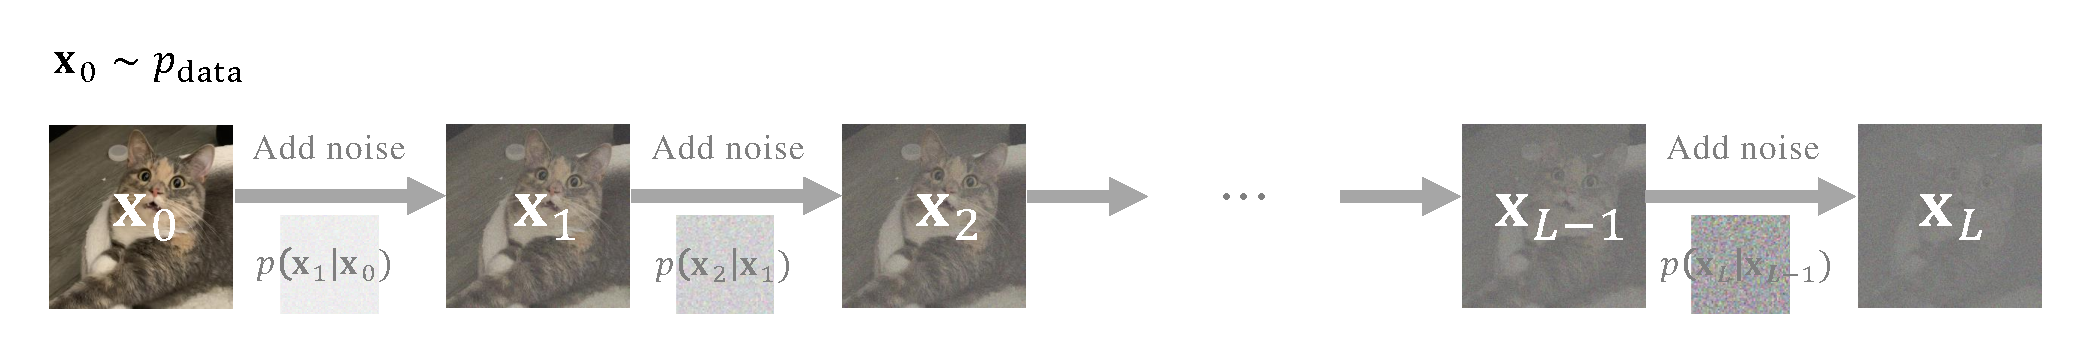
\includegraphics[width=\linewidth]{Images/PartB/vdm-forward.pdf}
    \caption{DDPM 前向过程的图示，其中增量添加高斯噪声以将数据样本破坏为纯噪声。 \figcredit{由作者创建。}}
    \label{fig:vdm-forward}
\end{figure}



让我们将这种逐步退化形式化：
\paragraph{固定高斯跃迁。}
前向过程中的每一步都由固定的高斯转移核控制\footnote{此公式虽然可能看起来不同，但在数学上等同于原始 DDPM 转换内核。}:
\[
p(\rvx_i|\rvx_{i-1}) := \mathcal{N}(\rvx_i; \sqrt{1 - \beta_i^2}   \rvx_{i-1}, \beta_i^2 \rmI).
\]
这里，过程开始于 $\rvx_{0} $，代表从真实数据分布中抽取的样本 $p_{\text{data}}$。顺序 $\{\beta_i\}_{i=1}^L$ 表示预先确定的、单调递增的噪声表，其中每个 
$\beta_i \in (0, 1)$ 控制步骤注入的高斯噪声的方差 $i$。为了方便起见，我们定义 $\alpha_i := \sqrt{1 - \beta_i^2}$。这个数学定义正好等价于下面直观的迭代更新：
\[
\rvx_i = \alpha_i \rvx_{i-1} + \beta_i \bm{\epsilon}_i,  
\]
哪里 $\bm{\epsilon}_i \sim \mathcal{N}(\bm{0}, \rmI)$ 独立同分布。这意味着在每一步 $i$，我们缩小之前的状态 $\rvx_{i-1}$ 通过 $\alpha_i$ 并添加按比例缩放的受控高斯噪声量 $\beta_i$.

\paragraph{扰动核和先验分布。}
通过递归应用转换内核，我们获得了噪声样本分布的封闭式表达式 $i$ 给出原始数据 $\rvx_0$:
\[
p_i(\rvx_i|\rvx_0) = \mathcal{N}\left(\rvx_i; \bar{\alpha}_i \rvx_0, (1 - \bar{\alpha}_i^2) \rmI \right),
\]
哪里 
\[
\bar{\alpha}_i := \prod_{k=1}^i \sqrt{1-\beta_k^2} = \prod_{k=1}^i \alpha_k.
\]
这意味着我们可以采样 $\rvx_i$ 直接来自 $\rvx$ 如
\begin{align}\label{eq:ddpm-forward}
    \rvx_i = \bar{\alpha}_i \rvx_0 + \sqrt{1-\bar{\alpha}_i^2}   \bm{\epsilon}, \quad \bm{\epsilon} \sim \mathcal{N}(\bm{0}, \rmI).
\end{align}
让噪音时间表 $ \{\beta_i\}_{i=1}^L $ 是一个递增序列，则前向过程的边缘分布收敛为
\[
p_L(\mathbf{x}_L | \rvx_0) \longrightarrow \mathcal{N}(\mathbf{0}, \mathbf{I}) \quad \text{as } L \to \infty,
\]
这促使选择先验分布为
\[
p_{\text{prior}} := \mathcal{N}(\mathbf{0}, \mathbf{I})
\]
不依赖数据 $\rvx_0$.










\subsection{反向去噪过程（可学习解码器）}



DDPM 的核心本质在于它们能够 \emph{反向} 前向扩散过程造成的受控退化。从纯粹的非结构化噪声开始， $\mathbf{x}_L \sim p_{\text{prior}}$，目标是逐步 \emph{降噪} 这种随机性，一步一步，直到出现连贯且有意义的数据样本。这种反向生成通过马尔可夫链进行，如下所示 \Cref{fig:ddpm-sampling-formal-rev}.
\begin{figure}[tbh!]
    \centering
    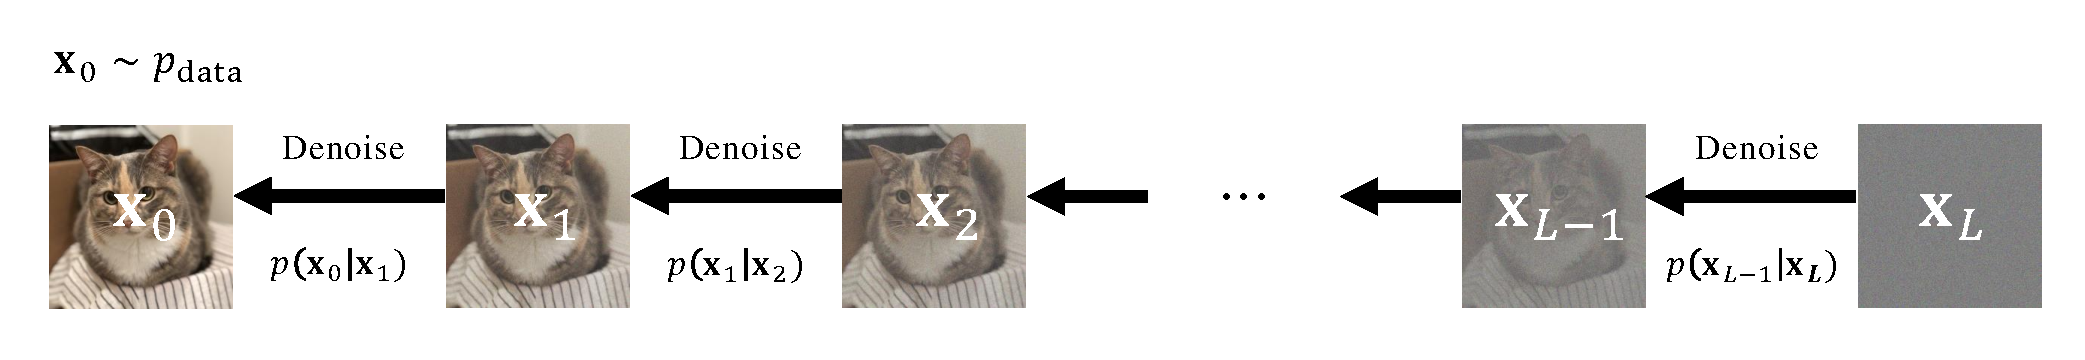
\includegraphics[width=\linewidth]{Images/PartB/vdm-backward.pdf}
\caption{\textbfs{DDPM 逆向（去噪）过程的图示。} 从噪音开始 $\mathbf{x}_L \sim  p_{\mathrm{prior}}$，模型顺序采样 $\mathbf{x}_{i-1} \sim  p(\mathbf{x}_{i-1}|\mathbf{x}_i)$ 用于 $i=L,\ldots,1$ 获取新生成的数据 $\mathbf{x}_0$。甲骨文的转变 $p(\mathbf{x}_{i-1}|\mathbf{x}_i)$ 未知；因此，我们的目标是对其进行近似。
\figcredit{由作者创建。}
}

    \label{fig:ddpm-sampling-formal-rev}
\end{figure}





指导 DDPM 开发的根本挑战和核心问题就变成了：
\begin{question}
我们能否精确计算或至少有效地近似这些反向转换内核 $ p(\mathbf{x}_{i-1}|\mathbf{x}_i) $，特别是考虑到复杂的分布时 $\mathbf{x}_i \sim p_i(\mathbf{x}_i)$?
\end{question}

而不是像最初的 DDPM 论文那样立即深入研究证据下界 (ELBO) 的数学上复杂的推导（对此有待详细讨论） \Cref{subsec:ddpm-elbo}），我们将从更直观的角度来实现训练目标：通过利用条件概率来实现易于处理的公式。 


\paragraph{概述：建模和训练目标。} 
为了启用生成过程，我们的目标是逼近未知的真实反向转换内核， $p(\mathbf{x}_{i-1}|\mathbf{x}_i)$。我们通过引入可学习的参数模型来实现这一目标， $p_{\bm{\phi}}(\mathbf{x}_{i-1}|\mathbf{x}_i)$，并训练它以最小化预期的 KL 散度：
\begin{align}\label{eq:marginal-kl-matching}
    \mathbb{E}_{p_i(\mathbf{x}_i)} \left[
    \mathcal{D}_{\mathrm{KL}}\big(p(\mathbf{x}_{i-1}|\mathbf{x}_i) \| p_{\bm{\phi}}(\mathbf{x}_{i-1}|\mathbf{x}_i)\big)
    \right].
\end{align}

但是，目标分布的直接计算 $p(\mathbf{x}_{i-1}|\mathbf{x}_i)$ 具有挑战性。根据贝叶斯定理，我们需要评估：
\[
p(\mathbf{x}_{i-1}|\mathbf{x}_i) = p(\mathbf{x}_i|\mathbf{x}_{i-1}) \underbrace{\frac{p_{i-1}(\mathbf{x}_{i-1})}{p_i(\mathbf{x}_i)}}_{\text{intractable}}.
\]
边缘 $p_i(\rvx_i)$ 和 $p_{i-1}(\rvx_{i-1})$ 是对未知数据分布的期望 $p_{\mathrm{data}}$，由下式给出：
\[
p_i(\rvx_i) = \int p_i(\rvx_i | \rvx_0) p_{\mathrm{data}}(\rvx_0) \mathrm{d}\rvx_0,
\]
类似地 $p_{i-1}(\rvx_{i-1})$。自从 $p_{\mathrm{data}}$ 未知，这些积分没有封闭式评估；充其量可以从样本中得到近似值，因此在实践中无法获得确切的密度。\begin{figure}[th!]
    \centering
    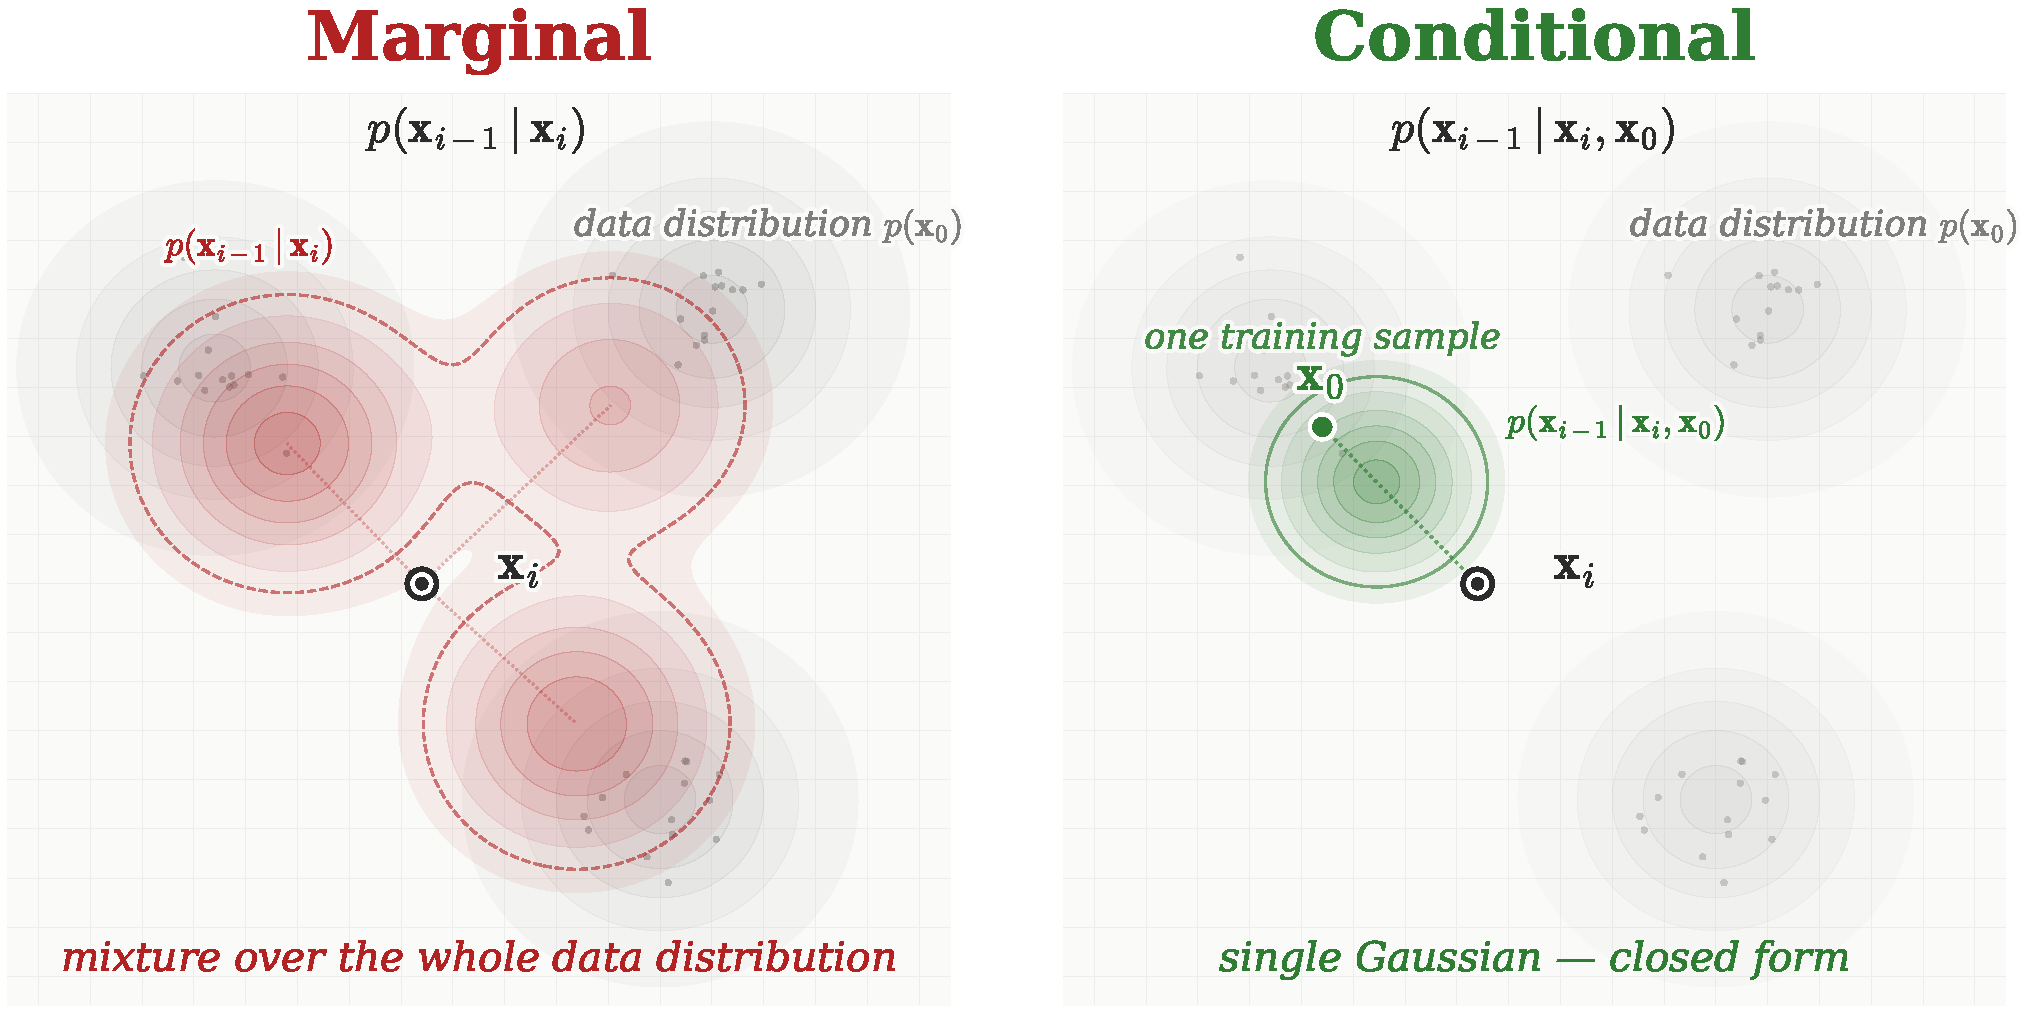
\includegraphics[width=\linewidth]{Images/PartB/ddpm_conditional_trick.pdf}
    \caption{\textbfs{DDPM中的调节技巧。}
\textbfs{(左)}
对于固定噪声样本 $\rvx_i$，逆分布
$p(\rvx_{i-1}|\rvx_i)$ 对所有可能的干净样品进行平均
$\rvx_0$ 可能会产生 $\rvx_i$。因此它可以是一个
复杂的混合物。
\textbfs{(右)}
然而，在训练期间，干净的样本 $\rvx_0$ 用于生成
$\rvx_i$ 是已知的。对该样本进行调节给出
$p(\rvx_{i-1}|\rvx_i,\rvx_0)$，具有闭合形式均值和的高斯
方差。因此，DDPM 可以使用这种易于处理的条件分布
作为简单的回归目标。虽然每个训练示例条件
仅在一个干净样本上，对条件训练目标进行平均
在所有样本上给出与直接学习相同的最佳模型
边缘逆分布；参见定理~\ref{thm:equiv-marginal-kl}。
因此，DDPM可以学习相同的最优反向预测，而无需直接
回归到复杂的、通常难以处理的目标
边缘混合物。    \figcredit{由作者使用AI辅助编码创建。}}
    \label{fig:conditional-trick}
\end{figure}


\paragraph{通过调节克服难处理性。}
DDPM 的核心见解解决了这个棘手问题：我们在干净的数据样本 $\mathbf{x}_0$ 上进行反向转换。这一微妙而强大的步骤将难以处理的内核转变为数学上易于处理的内核：
\[
p(\mathbf{x}_{i-1}|\mathbf{x}_i, \mathbf{x}_0) = p(\mathbf{x}_i|\mathbf{x}_{i-1}) \frac{p(\mathbf{x}_{i-1}|\mathbf{x}_0)}{p_i(\mathbf{x}_i|\mathbf{x}_0)}.
\]
这种易处理性源自前向过程的两个关键属性：其马尔可夫属性，即 $p(\mathbf{x}_i|\mathbf{x}_{i-1}, \mathbf{x}_0) = p(\mathbf{x}_i|\mathbf{x}_{i-1})$，以及所有涉及的分布的高斯性质。因此，$p(\mathbf{x}_{i-1}|\mathbf{x}_i, \mathbf{x}_0)$ 本身是高斯分布的，并且允许一个封闭式表达式（我们将在 \Cref{eq:ddpm-reverse-mean} 中看到）。我们将其可视化为 \Cref{fig:conditional-trick}。至关重要的是，这种优雅的调节策略使我们能够得出一个易于处理的目标，该目标在功能上相当于 \Cref{eq:marginal-kl-matching} 中看似棘手的边缘 KL 散度。

\thmp{边缘和条件 KL 最小化之间的等价}{equiv-marginal-kl}{
以下等式成立：
\begin{align}\label{eq:kl-matching}
\begin{aligned}
    &\mathbb{E}_{p_i(\rvx_i)}\left[
        \mathcal{D}_{\mathrm{KL}}\big(p(\rvx_{i-1}|\rvx_i) \| p_{\bm{\phi}}(\rvx_{i-1}|\rvx_i)\big)
    \right] \\
    ={}&
    \mathbb{E}_{p_{\mathrm{data}}(\rvx_0)}
    \mathbb{E}_{p_i(\rvx_i|\rvx_0)} \left[
        \mathcal{D}_{\mathrm{KL}}\big(p(\rvx_{i-1}|\rvx_i, \rvx_0) \| p_{\bm{\phi}}(\rvx_{i-1}|\rvx_i)\big)
    \right] + C.
\end{aligned}
\end{align}
其中 $C$ 是独立于 $\bm{\phi}$ 的常数。此外，\Cref{eq:kl-matching}的最小化器满足
\[
p^*(\mathbf{x}_{i-1}|\mathbf{x}_i) = \mathbb{E}_{p(\mathbf{x}_0|\mathbf{x}_i)} \big[p(\mathbf{x}_{i-1}|\mathbf{x}_i, \mathbf{x}_0)\big] = p(\mathbf{x}_{i-1}|\mathbf{x}_i), \quad \mathbf{x}_i \sim p_i.
\]
}{该证明通过扩展定义、应用概率链式法则并使用对数恒等式将其分解为预期条件 KL 散度和边缘 KL 散度之和，重写了 KL 散度期望。完整的推导在\Cref{subsec:proof-equiv-marginal-kl}.}


这种替代观点：调节以获得易于处理的目标，构成了 DDPM 的基础，并揭示了与其他有影响力的扩散模型的深刻共性，正如我们将在 \Cref{ch:score-based} 和 \Cref{ch:flow-based} 中探讨的那样。

它揭示了一个强大的等价性：最小化边缘分布之间的 KL 散度在数学上与最小化特定条件分布之间的 KL 散度相同。后一个公式非常有用，因为关键的条件分布， $p(\mathbf{x}_{i-1}|\mathbf{x}_i, \mathbf{x})$，具有方便的封闭式表达式：
\lem{反向条件转换内核}{ddpm-reverse-kernel}{$p(\mathbf{x}_{i-1} | \mathbf{x}_i, \mathbf{x})$ 是高斯分布，其封闭式表达式为：
\begin{align*}
    p(\rvx_{i-1} | \rvx_i, \rvx) =\mathcal{N}\left(\rvx_{i-1}; \bm{\mu}\left(\rvx_i, \rvx, i\right), \sigma^2(i)\rmI \right),
\end{align*}
哪里
\begin{align}\label{eq:ddpm-reverse-mean}
\begin{aligned}
            \bm{\mu}\left(\rvx_i, \rvx, i\right):= \frac{\bar{\alpha}_{i-1}\beta_i^2}{1-\bar{\alpha}_i^2}\rvx + \frac{(1-\bar{\alpha}_{i-1}^2)\alpha_i }{1-\bar{\alpha}_i^2}\rvx_i,
\quad  \sigma^2(i) := \frac{1-\bar{\alpha}_{i-1}^2}{1-\bar{\alpha}_i^2}\beta_i^2.
\end{aligned}
\end{align}
}
稍后在引理中~\ref{reverse-kernel}，我们提出了一个更通用的公式，该公式超出了 DDPM 噪声过程中描述的范围 \Cref{eq:ddpm-forward}.


\subsection{反向转换内核的建模 $p_{\bm{\phi}}(\mathbf{x}_{i-1}|\mathbf{x}_i)$} 利用定理中的梯度级等价~\ref{thm:equiv-marginal-kl} 以及相反条件的高斯形式 $p(\mathbf{x}_{i-1}|\mathbf{x}_i, \mathbf{x})$ 如引理中所示~\ref{ddpm-reverse-kernel}，DDPM 假设每个反向转换 $p_{\bm{\phi}}(\rvx_{i-1}| \rvx_i)$ 为高斯分布，参数化为
\begin{align}\label{eq:def-reverse}
    p_{\bm{\phi}}(\mathbf{x}_{i-1}|\mathbf{x}_i) := \mathcal{N}\big(\mathbf{x}_{i-1}; \bm{\mu}_{\bm{\phi}}(\mathbf{x}_i, i), \sigma^2(i) \mathbf{I}\big),
\end{align}
哪里 $\bm{\mu}_{\bm{\phi}}(\cdot, i) \colon \mathbb{R}^D \to \mathbb{R}^D$ 是一个可学习的均值函数，并且 $\sigma^2(i) > 0$ 按照中的定义进行固定 \Cref{eq:ddpm-reverse-mean}。我们表示 KL 散度，在时间步长上取平均值 $i$ 并以数据为条件 $\rvx_0 \sim p_{\text{data}}$，将所有分布层匹配为：
\begin{align}\label{eq:ddpm-diffusion}
    \mathcal{L}_{\text{diffusion}}(\rvx_0;\bm{\phi}) := \sum_{i=2}^L \mathbb{E}_{p_i(\rvx_i|\rvx_0)}\left[\mathcal{D}_{\text{KL}}\big(p(\rvx_{i-1}|\rvx_i, \rvx_0)  \Vert  p_{\bm{\phi}}(\rvx_{i-1}|\rvx_i)\big)\right].
\end{align}
得益于两种分布的高斯形式以及中定义的参数化 \Cref{eq:def-reverse}，目标允许封闭式表达式，可以简化为：
\begin{align}\label{eq:ddpm-diffusion-simp}
    \mathcal{L}_{\text{diffusion}}(\rvx_0;\bm{\phi}) = \sum_{i=2}^L \frac{1}{2\sigma^2(i)}  \mathbb{E}_{p_i(\rvx_i|\rvx_0)}\left\| \bm{\mu}_{\bm{\phi}}(\rvx_i, i) - \bm{\mu}(\rvx_i, \rvx_0, i) \right\|_2^2 + C,
\end{align}
哪里 $C$ 是一个独立于 $\bm{\phi}$。对数据分布求平均值并忽略常数 $C$ （不影响优化），最终的DDPM训练目标是
\begin{align}
\begin{aligned}
    \label{eq:ddpm-mean-loss}
    \mathcal{L}_{\text{DDPM}}(\bm{\phi}) := \sum_{i=2}^L \frac{1}{2\sigma^2(i)}  \mathbb{E}_{\rvx_0} \mathbb{E}_{p_i(\rvx_i|\rvx_0)} \left[ \left\| \bm{\mu}_{\bm{\phi}}(\mathbf{x}_i, i) - \bm{\mu}(\mathbf{x}_i, \rvx_0, i) \right\|_2^2 \right],
\end{aligned}
\end{align}
哪里 $\rvx_0\sim p_{\mathrm{data}}$。我们注意到前向扰动核 $p_i(\rvx_i | \rvx_0)
$
在训练目标中起着重要的计算作用。它给出了噪声状态的分布 $\rvx_i$ 从干净的样品中获得 $\rvx_0$
之后 $i$ 向前迈出一步。由于每个前向过渡都是线性且高斯分布的，因此它们的组成也具有闭合形式的高斯分布；请参阅周围的讨论 \Cref{eq:ddpm-forward}。因此，选择时间步后 $i$，我们可以取样 $\rvx_i \sim p_i(\rvx_i | \rvx_0)
$
直接来自 $\rvx_0$，没有首先生成中间状态
$\rvx_1,\ldots,\rvx_{i-1}$。因此，每个损失项可以仅使用干净的样本、选定的时间步长和直接损坏的样本来估计，从而使随机训练的计算效率更高。


\subsection{预测和损失的实用选择}\label{subsec:ddpm-prediction}

\paragraph{$\beps$-预测。}
在典型的 DDPM 实现中，不会直接使用基于 \emph{均值预测} 参数化来自 \Cref{eq:ddpm-mean-loss}。相反，等效的重新参数化，称为 \emph{$\beps$-预测} （噪声预测）表述，普遍采用。  

回想一下，在 DDPM 前向过程中，噪声样本 $\rvx_i \sim p(\rvx_i |\rvx_0)$ 处于噪声水平 $i$ 由生成
\begin{equation}\label{eq:ddpm-perturbation}
    \rvx_i = \bar{\alpha}_i \rvx_0 + \sqrt{1 - \bar{\alpha}_i^2}   \boldsymbol{\epsilon}, \quad \rvx_0 \sim p_{\text{data}}, \quad \boldsymbol{\epsilon} \sim \mathcal{N}(\mathbf{0}, \mathbf{I}).
\end{equation}
使用这个表达式，相反的意思 $\bm{\mu}(\rvx_i, \rvx_0, i)$ 来自 \Cref{eq:ddpm-reverse-mean} 可以重写为：
\[
\bm{\mu}(\rvx_i, \rvx_0, i) = \frac{1}{\alpha_i} \left( \rvx_i - \frac{1 - \alpha_i^2}{\sqrt{1 - \bar{\alpha}_i^2}} \boldsymbol{\epsilon} \right).
\]

这激发了模型均值的参数化 $\bm{\mu}_{\bm{\phi}}$ 使用神经网络 $\boldsymbol{\epsilon}_{\bm{\phi}}(\rvx_i, i)$ 直接预测噪声：
\[
\bm{\mu}_{\bm{\phi}}(\rvx_i, i) = \frac{1}{\alpha_i} \left( \rvx_i - \frac{1 - \alpha_i^2}{\sqrt{1 - \bar{\alpha}_i^2}} \underbrace{\boldsymbol{\epsilon}_{\bm{\phi}}(\rvx_i, i)}_{\beps\text{-prediction}} \right).
\]
将其代入原始损失，得到平方 $\ell_2$ 预测噪声和真实噪声之间的误差：
\[
\left\| \bm{\mu}_{\bm{\phi}}(\rvx_i, i) - \bm{\mu}(\rvx_i, \rvx_0, i) \right\|_2^2 \propto \left\| \boldsymbol{\epsilon}_{\bm{\phi}}(\rvx_i, i) - \boldsymbol{\epsilon} \right\|_2^2,
\]
权重因子取决于 $i$。直观地说，该模型充当“噪声侦探”，估计在前向过程的每个步骤中添加的随机噪声。从损坏的样本中减去该估计值，使其更接近干净的原始样本，并逐步重复此操作，从纯噪声中重建数据。

\paragraph{简化损失 $\beps$-预测。}
实际上，通过省略权重项，可以进一步简化该表达式，从而产生广泛使用的 DDPM 训练损失：
\begin{equation}\label{eq:ddpm-simple-loss}
    \mathcal{L}_{\text{simple}}(\bm{\phi}) := \mathbb{E}_{i} \mathbb{E}_{\rvx \sim p_{\text{data}}(\rvx)} \mathbb{E}_{\boldsymbol{\epsilon} \sim \mathcal{N}(\mathbf{0}, \mathbf{I})} \left[ \left\| \boldsymbol{\epsilon}_{\bm{\phi}}(\rvx_i, i) - \boldsymbol{\epsilon} \right\|_2^2 \right],
\end{equation}
哪里 $\rvx_i = \bar{\alpha}_i \rvx_0 + \sqrt{1 - \bar{\alpha}_i^2} \boldsymbol{\epsilon}$ 与 $\rvx_0 \sim p_{\text{data}}$。由于目标噪声在每个时间步长都有单位方差 $t$， $\ell_2$ 损失 \Cref{eq:ddpm-simple-loss} 在所有方面保持一致的规模 $t$。这可以防止目标消失或爆炸，并消除显式损失加权的需要。重要的是，两者 $\mathcal{L}_{\text{DDPM}}$ 和 $\mathcal{L}_{\text{simple}}$ 共享相同的最优解 $\boldsymbol{\epsilon}^*$，这是因为 \Cref{eq:ddpm-simple-loss} 本质上简化为最小二乘问题（如命题中类似所示）~\ref{dsm-minimizer} 或提议~\ref{equi-para})\footnote{我们注意到，删除了 ELBO 派生的权重 $\mathcal{L}_{\text{DDPM}}$ 更改训练目标，但不更改其群体最优预测： $\beps^*(\rvx_i,i)
=
\E[\beps| \rvx_i]$。因此，加权和简化的 DDPM 损失具有相同的理想预测器，但它们在训练期间强调不同的噪声水平。实际上，这种权重仍然会影响优化和性能。}:
\[
\boldsymbol{\epsilon}^*(\rvx_i, i) = \mathbb{E}\left[ \boldsymbol{\epsilon}|\rvx_i \right], \quad \rvx_i \sim p_i.
\]
直观地说， $\beps$-预测网络 $\boldsymbol{\epsilon}_{\bm{\phi}}(\rvx_i, i)$ 估计前向过程添加的噪声以产生 $\rvx_i$。在最优情况下，该估计与真实噪声的条件期望一致，即使 $\rvx_i$ 不能唯一确定原始干净样本。

\paragraph{另一个等效参数化： $\rvx$-预测。} 
\Cref{eq:ddpm-reverse-mean} 激发了一种替代但等效的参数化，称为 \emph{$\rvx$-预测} （干净的预测），其中一个神经网络 $\rvx_{\bm{\phi}}(\rvx_i, i)$ 经过训练，可以从给定的噪声输入中预测干净（去噪）的样本 $\rvx_i \sim p_i(\rvx_i)$ 处于噪声水平 $i$。替换真实的干净样本 $\rvx_0$ 在反向均值表达式中 $\rvx_{\bm{\phi}}(\rvx_i, i)$ 导致以下模型：
\begin{align*}
\bm{\mu}_{\bm{\phi}}(\rvx_i, i) = \frac{\bar{\alpha}_{i-1} \beta_i^2}{1 - \bar{\alpha}_i^2} \rvx_{\bm{\phi}}(\rvx_i, i) + \frac{(1 - \bar{\alpha}_{i-1}^2)\alpha_i}{1 - \bar{\alpha}_i^2} \rvx_i.
\end{align*}
类似于 $\beps$-预测公式，训练目标可以表示为
\[
\left\| \bm{\mu}_{\bm{\phi}}(\rvx_i, i) - \bm{\mu}(\rvx_i, \rvx_0, i) \right\|_2^2 \propto \left\| \rvx_{\bm{\phi}}(\rvx_i, i) - \rvx_0 \right\|_2^2, \quad \rvx_0 \sim p_{\text{data}},
\]
训练模型来预测原始数据样本 $\rvx_0$ 来自其嘈杂的版本 $\rvx_i$。这种等价性减少了均值匹配损失 \Cref{eq:ddpm-mean-loss} 至
\[
\mathbb{E}_{i} \mathbb{E}_{\rvx_0 \sim p_{\text{data}}} \mathbb{E}_{\boldsymbol{\epsilon} \sim \mathcal{N}(\mathbf{0}, \mathbf{I})} \left[\omega_i \left\| \rvx_{\bm{\phi}}(\rvx_i, i) - \rvx_0 \right\|_2^2 \right],
\]
用于某些加权函数 $\omega_i$。由于这是一个最小二乘问题，因此最优解由下式给出（参见命题~\ref{dsm-minimizer} 或提议~\ref{equi-para}) 
\begin{align}\label{eq:ddpm-clean-minimizer}
    \rvx^*(\rvx_i, i) = \mathbb{E}\left[ \rvx_0|\rvx_i \right], \quad \rvx_i \sim p_i,
\end{align}
也就是说，模型应该在给定噪声观察的情况下预测预期的干净数据 $\rvx_i$ 在时间步长 $i$。的 $\rvx$-预测和 $\beps$-预测参数化在数学上是等效的并且通过前向过程连接：
\begin{equation}\label{eq:ddpm-clean-noise}
    \rvx_i = \bar{\alpha}_i \rvx_{\bm{\phi}}(\rvx_i, i) + \sqrt{1 - \bar{\alpha}_i^2}   \boldsymbol{\epsilon}_{\bm{\phi}}(\rvx_i, i).
\end{equation}
也就是说，人们可以预测干净的样本 $\rvx_{\bm{\phi}}(\rvx_i, i)$ 或者噪音 $\boldsymbol{\epsilon}_{\bm{\phi}}(\rvx_i, i)$，这样它们的组合就会重现 $\rvx_i$ 在前向噪声过程下。 




\subsection{DDPM的ELBO}\label{subsec:ddpm-elbo} 反向转换定义如下 \Cref{eq:def-reverse}，这导致 DDPM 中联合生成分布的定义为：
\[
p_{\bm{\phi}}(\rvx_0, \rvx_{1:L}) := p_{\bm{\phi}}(\rvx_0|\rvx_1)  p_{\bm{\phi}}(\rvx_1|\rvx_2)\cdots p_{\bm{\phi}}(\rvx_{L-1}|\rvx_L)   p_{\text{prior}}(\rvx_L),
\]
数据的边缘生成模型由下式给出：
\begin{align*}
    p_{\bm{\phi}}(\rvx_0) := \int p_{\bm{\phi}}(\rvx_0, \rvx_{1:L}) \diff \rvx_{1:L}.
\end{align*}

确实，DDPM 训练通过 \Cref{eq:ddpm-diffusion} 可以严格基于最大似然估计（\Cref{eq:MLE}）。具体来说，它的目标形成了 ELBO，类似于 VAE 和 HVAE 中的目标 \Cref{sec:vae}，用作对数密度的下限：
\thmp{DDPM的ELBO}{ddpm-elbo}{    
\begin{align}\label{eq:ddpm-elbo}
        \begin{aligned}
        -\log p_{\bm{\phi}}(\rvx_0)  &\leq-\mathcal{L}_{\text{ELBO}}(\rvx_0; \bm{\phi}) 
        \\&:= \mathcal{L}_{\text{prior}}(\rvx_0) + \mathcal{L}_{\text{recon.}}(\rvx_0;\bm{\phi})  + \mathcal{L}_{\text{diffusion}}(\rvx_0;\bm{\phi})
        \end{aligned}
\end{align}
这里，损耗的每个组成部分定义为：
\begin{align*}
   \mathcal{L}_{\text{prior}}(\rvx_0) &:= \mathcal{D}_{\text{KL}}\Big( p(\rvx_L|\rvx_0) \Vert p_{\text{prior}}(\rvx_L)\Big)\\
   \mathcal{L}_{\text{recon.}}(\rvx_0;\bm{\phi}) &:= \mathbb{E}_{p(\rvx_1|\rvx_0)}\left[-\log p_{\bm{\phi}}(\rvx_0|\rvx_1)\right]\\
   \mathcal{L}_{\text{diffusion}}(\rvx_0;\bm{\phi}) &= \sum_{i=2}^L  \mathbb{E}_{p_i(\rvx_i|\rvx_0)}\left[\mathcal{D}_{\text{KL}}\Big(p(\rvx_{i-1}|\rvx_i, \rvx_0) \Vert p_{\bm{\phi}}(\rvx_{i-1}|\rvx_i) \Big)\right]. 
\end{align*}}{推导应用 Jensen 不等式，如 HVAE/VAE ELBO 中所示（\Cref{eq:hvae-elbo})，进一步简化。详细证明推迟到 \Cref{app:vlb-proof}.
}
ELBO $\mathcal{L}_{\text{ELBO}}$ 由三个术语组成：
\begin{itemize}
    \item $\mathcal{L}_{\text{prior}}$ 通过选择噪声表可以忽略不计 $\{\beta_i\}$ 这样 $p(\cdot|\rvx_0) \approx p_{\text{prior}}(\cdot)$.
    \item 对于 $\mathcal{L}_{\text{recon.}}$，这可以使用蒙特卡洛估计进行近似和优化；看到 \citep{ho2020denoising, kingma2021variational} 用于实际实现。 
    \item $\mathcal{L}_{\text{diffusion}}$ （参见 \Cref{eq:ddpm-diffusion}) 匹配反向条件 $p_{\bm{\phi}}(\mathbf{x}_{i-1}|\mathbf{x}_i)$ 到 $p(\mathbf{x}_{i-1}|\mathbf{x}_i)$ 在所有步骤 $i$.
\end{itemize}

ELBO 物镜 $\mathcal{L}_{\text{ELBO}}$ 也可以通过潜在的数据处理不等式的镜头来解释 $\rvz = \rvx_{1:L}$，如图所示 \Cref{eq:joint-bound}:
\begin{align*}
    \mathcal{D}_{\mathrm{KL}}(p_{\mathrm{data}}(\rvx_0) \| p_{\bm{\phi}}(\rvx_0)) \leq \mathcal{D}_{\mathrm{KL}}\left(p(\rvx_0, \rvx_{1:L}) \| p_{\bm{\phi}}(\rvx_0, \rvx_{1:L})\right),
\end{align*}
哪里 $p(\rvx_0, \rvx_{1:L}) := p_{\mathrm{data}}(\rvx_0)  p(\rvx_1|\rvx_0)  p(\rvx_2|\rvx_1) \cdots p(\rvx_L|\rvx_{L-1})$ 表示沿前向过程的联合分布。 



\rmkb{扩散的变分视图以一种特别方便的方式拟合分层潜变量图：“编码器”是固定的前向噪声链，因此没有学习的推理网络。尽管如此，ELBO 确实分解为每步 KL 项，以及最终先验项和重构项 \Cref{eq:ddpm-elbo}。 DDPM 训练特别容易处理的原因是，在线性高斯前向过程下，这些每步 KL 项可以重写为具有封闭形式条件目标的简单去噪回归问题。因此，关键的简化不是缺少每级 KL 项，而是前向过程是固定的，并将它们转变为可以有效采样的监督去噪目标。}





\subsection{采样} 
训练后 $\beps$-预测模型， $\bm{\epsilon}_{\bm{\phi}^\times}(\rvx_i, i)$\footnote{我们使用符号``$\times$'' 表示模型已经过训练并且现在被冻结。}，采样按顺序执行，如图所示 \Cref{fig:ddpm-sampling-formal-rev}，使用参数化过渡 $p_{\bm{\phi}^\times}(\rvx_{i-1} | \rvx_i)$ 相反。更具体地说，从随机种子开始 $\rvx_L \sim p_{\text{prior}} = \mathcal{N}(\bm{0},\rmI)$，我们递归地采样 $p_{\bm{\phi}^\times}(\rvx_{i-1} | \rvx_i)$ 遵循以下更新规则 $i = L, L-1, \dots, 1$:
\begin{align}\label{eq:ddpm-sampling}
    \rvx_{i-1} \leftarrow \underbrace{\frac{1}{\alpha_i}\left( \rvx_i  - \frac{1-\alpha_i^2}{\sqrt{1-\bar{\alpha}_i^2}} \bm{\epsilon}_{\bm{\phi}^\times}(\rvx_i, i)\right)}_{\bm{\mu}_{\bm{\phi}^\times}(\rvx_i, i)} +\sigma(i) \bm{\epsilon}_i,\quad \bm{\epsilon}_i\sim  \mathcal{N}(\bm{0},\rmI).
\end{align}
这个“降噪”过程一直持续到 $\rvx_0$ 作为最终干净生成的样本获得。 















































\paragraph{DDPM 采样的另一种解释。}

解释 DDPM 采样的一个有用方法是重写更新规则，以便噪声级别结构变得明确。回忆起 \Cref{eq:ddpm-clean-noise} 预测噪声可以用当前样本来表示 $\rvx_i$ 以及预测的干净样本 $\rvx_{\bm{\phi}^\times}(\rvx_i,i)$:
\[
\boldsymbol{\epsilon}_{\bm{\phi}^\times}(\rvx_i,i)
=
\frac{\rvx_i - \bar{\alpha}_i\,\rvx_{\bm{\phi}^\times}(\rvx_i,i)}
     {\sqrt{1-\bar{\alpha}_i^2}}.
\]
将其代入 DDPM 采样规则（\Cref{eq:ddpm-sampling}) 并重新排列，我们得到
\begin{equation}\label{eq:ddpm-renoise}
\rvx_{i-1}
\;\leftarrow\;
\bar{\alpha}_{i-1}\,\rvx_{\bm{\phi}^\times}(\rvx_i,i)
\;+\;
\underbrace{
  \sqrt{1-\bar{\alpha}_{i-1}^2 - \tilde{\beta}_i^2}\;
  \boldsymbol{\epsilon}_{\bm{\phi}^\times}(\rvx_i,i)
  \;+\;
  \tilde{\beta}_i\,\boldsymbol{\epsilon}_i
}_{\text{combined std.\ }=\;\sqrt{1-\bar{\alpha}_{i-1}^2}},
\end{equation}
哪里 $\tilde{\beta}_i^2
= \frac{(1-\bar{\alpha}_{i-1}^2)(1-\alpha_i^2)}{1-\bar{\alpha}_i^2}$
是DDPM后验方差\footnote{
系数
$\sqrt{1-\bar{\alpha}_{i-1}^2 - \tilde{\beta}_i^2}$
简化为
$\frac{\alpha_i(1-\bar{\alpha}_{i-1}^2)}{\sqrt{1-\bar{\alpha}_i^2}}$，始终为非负数，因此平方根是明确定义的。}。此外，残差系数满足
\[
\bigl(1-\bar{\alpha}_{i-1}^2-\tilde{\beta}_i^2\bigr)+\tilde{\beta}_i^2
=
1-\bar{\alpha}_{i-1}^2,
\]
因此更新具有与 level 的前向边缘相同的噪声级别结构 $i-1$。这返回到中引入的第一个操作采样模板
\Cref{eq:ddpm-first-try}：预测干净部分并以较低噪声水平重写样本。 DDPM 随机地执行此重写，结合从以下位置估计的噪声方向 $\rvx_i$ 具有新的高斯噪声样本。确定性采样器遵循相同的基本思想，但消除了新的随机性并相应地调整剩余的噪声系数。当我们更系统地研究扩散采样器时，我们将重新审视这种结构 \Cref{sec:revisit-ddim}.

比较 \Cref{eq:ddpm-renoise} 具有前向边缘
$\rvx_{i-1} = \bar{\alpha}_{i-1}\,\rvx_0
+ \sqrt{1-\bar{\alpha}_{i-1}^2}\,\bar{\boldsymbol{\epsilon}}$。结构相同：信号系数 $\bar{\alpha}_{i-1}$
和噪声标准差 $\sqrt{1-\bar{\alpha}_{i-1}^2}$，除了未知 $\rvx_0$ 被网络预测取代 $\rvx_{\bm{\phi}^\times}(\rvx_i,i)$。换句话说，每个 DDPM 步骤 \emph{预测干净的数据，然后将其重新噪声化至精确的噪声水平 $i{-}1$}。因此，我们可以将 DDPM 采样视为迭代两个操作：
\begin{enumerate}
    \item \textbfs{降噪。}
          估计干净数据
          $\rvx_{\bm{\phi}^\times}(\rvx_i, i)$
          来自当前噪声输入 $\rvx_i$.
    \item \textbfs{重新噪音。}
          以降低的级别添加回噪 $i{-}1$
          通过 \Cref{eq:ddpm-renoise}，正在制作样品 $\rvx_{i-1}$ 其噪声水平与步骤中的前向过程匹配 $i{-}1$.
\end{enumerate}


但是，即使 $\rvx_{\bm{\phi}^\times}$ 被训练为最佳降噪器（即条件期望最小化器；参见 \Cref{eq:ddpm-clean-minimizer})，它只能预测
\emph{平均} 给出干净的样品 $\rvx_i$。这种限制导致预测模糊，特别是在高噪声水平下，从严重损坏的输入中恢复详细结构变得困难。从这个角度来看，扩散采样从高噪声转向低噪声，并逐渐完善对干净信号的估计。早期的步骤设置全局结构，后续的步骤添加精细的细节，并且随着噪声的去除，样本变得更加真实。



\begin{figure}[th!]
    \centering
    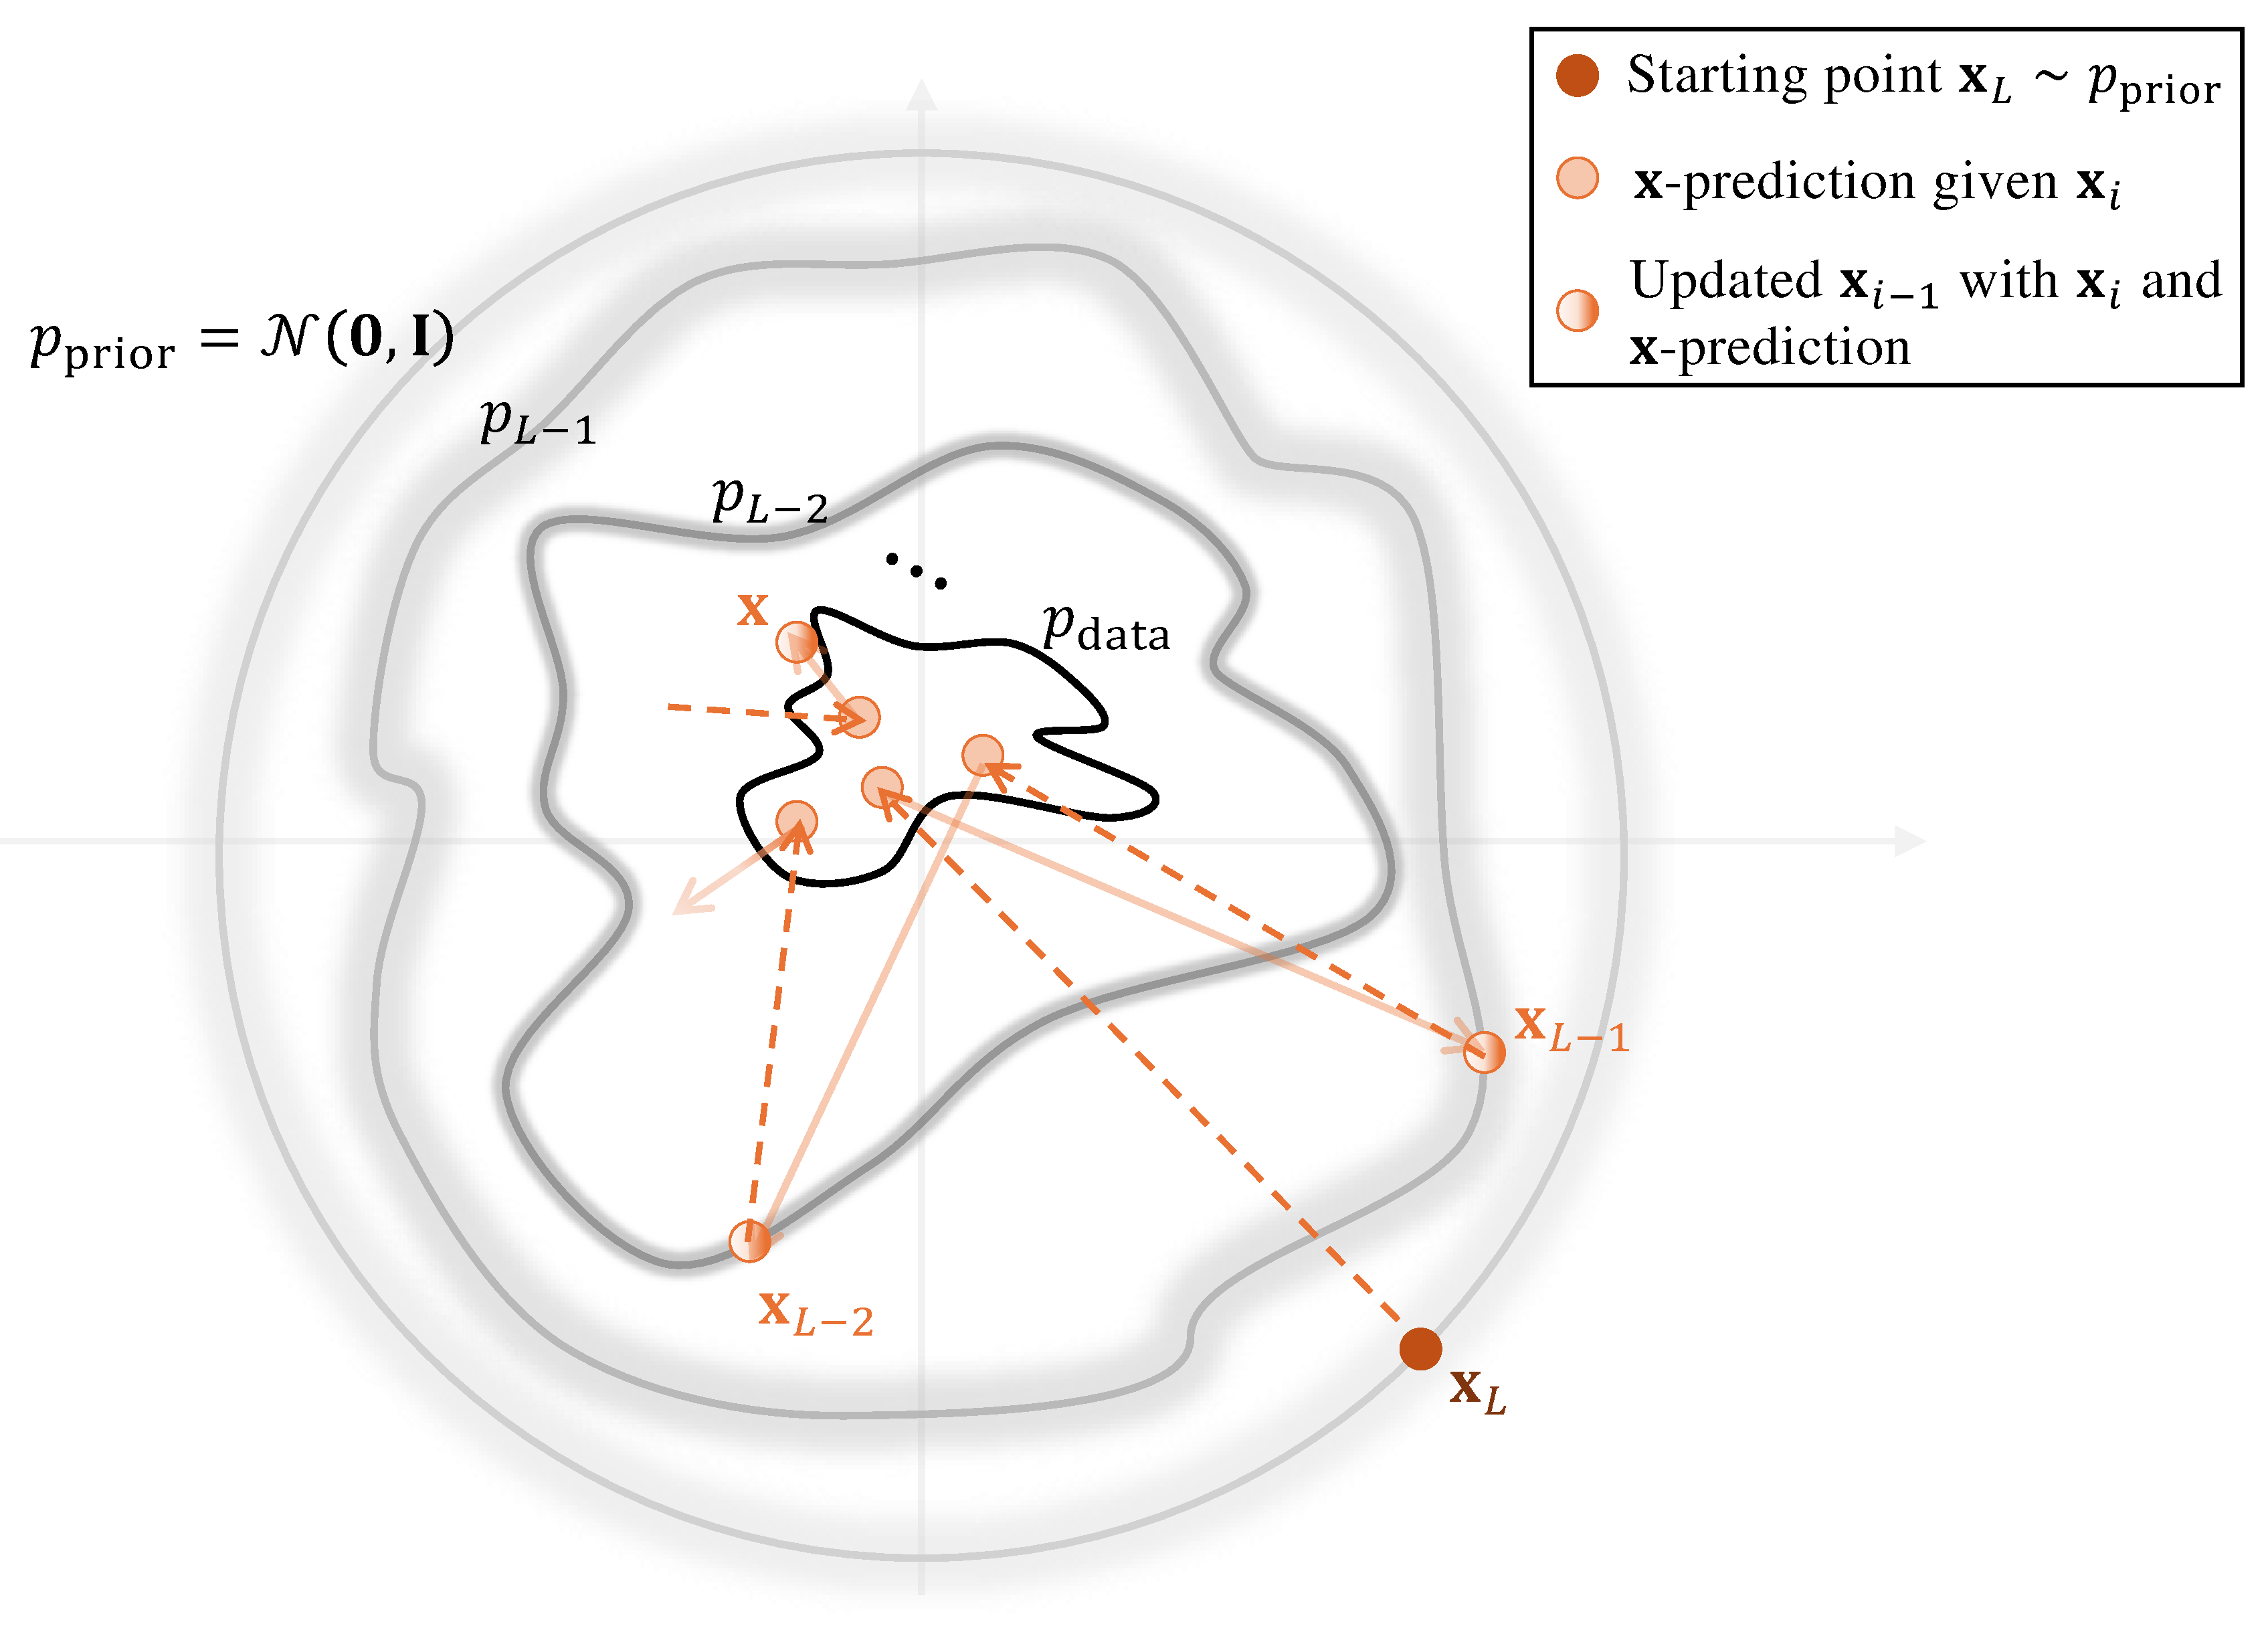
\includegraphics[width=\linewidth]{Images/PartB/diffusion-clean.pdf}
\caption{\textbfs{DDPM 采样的去噪然后再噪声视图的图示。} 来自当前噪声样本 $\mathbf{x}_i$，模型首先估计底层干净信号 $\mathbf{x}_{\bm{\phi}^\times}(\mathbf{x}_i,i)$，然后采样噪声较小的点 $\mathbf{x}_{i-1}$ 通过将该估计重新加噪 $(i-1)$第-噪声级。 \figcredit{由作者创建。}}
    \label{fig:vdm-clean}
\end{figure}



\paragraph{DDPM 采样速度慢。} DDPM（即扩散模型）中的采样本质上很慢。在最初的制定和实施中，生成样本通常需要大约 $1{,}000$ 去噪步骤。这是因为采样是通过一长串的小改进进行的：在每一步，模型都会将当前的噪声样本稍微更新为更干净的样本，并且下一次更新必须从上一步的结果开始。因此，标准 DDPM 采样是时间步进的且具有强顺序性，良好的样本质量通常需要许多这样的步骤来密切跟踪反向扩散路径。定理~\ref{thm:equiv-marginal-kl} 表明富有表现力 $ p_{\bm{\phi}}(\mathbf{x}_{i-1} | \mathbf{x}_i) $ 理论上可以匹配真实的反向分布 $ p(\mathbf{x}_{i-1} | \mathbf{x}_i) $。然而，在实践中， $ p_{\bm{\phi}}(\mathbf{x}_{i-1} | \mathbf{x}_i) $ 通常建模为高斯以近似 $ p(\mathbf{x}_{i-1} | \mathbf{x}_i) $，限制了它的表现力。对于小前向噪声尺度 $\beta_i$，真正的反向分布近似为高斯分布，从而实现精确逼近。相反，大的 $\beta_i$ 会导致多模态或强非高斯性，这是单个高斯函数无法捕获的。为了保持准确性，DDPM 采用许多小的 $\beta_i$ 步骤，形成一个顺序链，其中每个步骤都依赖于前一个步骤，并且需要神经网络评估 $\boldsymbol{\epsilon}_{\bm{\phi}^\times}(\mathbf{x}_i, i)$。这会导致 $\mathcal{O}(L)$ 顺序传递，从而阻止并行化并减慢生成速度。



后来在 \Cref{ch:score-sde} 中，我们展示了对这种固有采样瓶颈作为微分方程问题的更原则性解释，这激发了加速生成的连续时间数值策略。



\newpage
\section{结束语}\label{sec:ch2_cr}


在本章中，我们通过变分透镜追溯了扩散模型的起源。我们从变分自编码器 (VAE) 开始，这是一种基础生成模型，可通过证据下界 (ELBO) 学习数据与结构化潜在空间之间的概率映射。我们看到了分层 VAE (HVAE) 如何通过堆叠潜在层来扩展这一想法，引入渐进式、从粗到细生成的强大概念。然而，这些模型面临着训练稳定性和样本质量的挑战。





然后，我们将去噪扩散概率模型（DDPM）定义为该变分框架内的关键演变。通过将编码器固定为渐进的噪声过程并仅学习反向降噪步骤，DDPM 优雅地回避了 HVAE 的训练不稳定性。至关重要的是，我们证明了 DDPM 也是通过最大化对数似然的变分界限来训练的，训练目标可分解为一系列简单的去噪任务。这种易处理性是通过强大的调节策略实现的，该策略将棘手的边缘目标转化为易于处理的条件目标，这是扩散模型中反复出现的主题。





虽然这个变分框架为 DDPM 提供了完整而强大的基础，但它并不是理解它们的唯一方法。基于能量的建模原理出现了另一种同样基本的观点。在下一章中，我们将探讨这种基于分数的观点：
\begin{enumerate}
    \item 我们将把重点从学习去噪转移概率 $p_{\bm{\phi}}(\mathbf{x}_{i-1}\vert\mathbf{x}_{i})$ 转移到直接学习数据对数密度的梯度，即分数函数。
    \item 我们将看到这种源自 EBM 的方法如何产生噪声条件分数网络 (NCSN)，并揭示在 DDPM 中学习的噪声预测（$\bm{\epsilon}$ 预测）与评分函数本身之间的深层数学等价性。
\end{enumerate}

这种替代观点不仅会提供新的见解，而且可以作为后续开发的统一、连续时间扩散模型框架的另一个基石。